\hypertarget{protists}{%
\chapter{Protists}\label{protists}}

A \href{https://en.wikipedia.org/wiki/Protist}{protist} is any eukaryotic organism (one with cells containing a nucleus) that is not an animal, plant, or fungus. While it is likely that protists share a common ancestor (the last eukaryotic common ancestor), the exclusion of other eukaryotes means that protists do not form a natural group, or clade. So some protists may be more closely related to animals, plants, or fungi than they are to other protists; however, like algae, invertebrates, or protozoans, the grouping is used for convenience.



\begin{figure}

{\centering 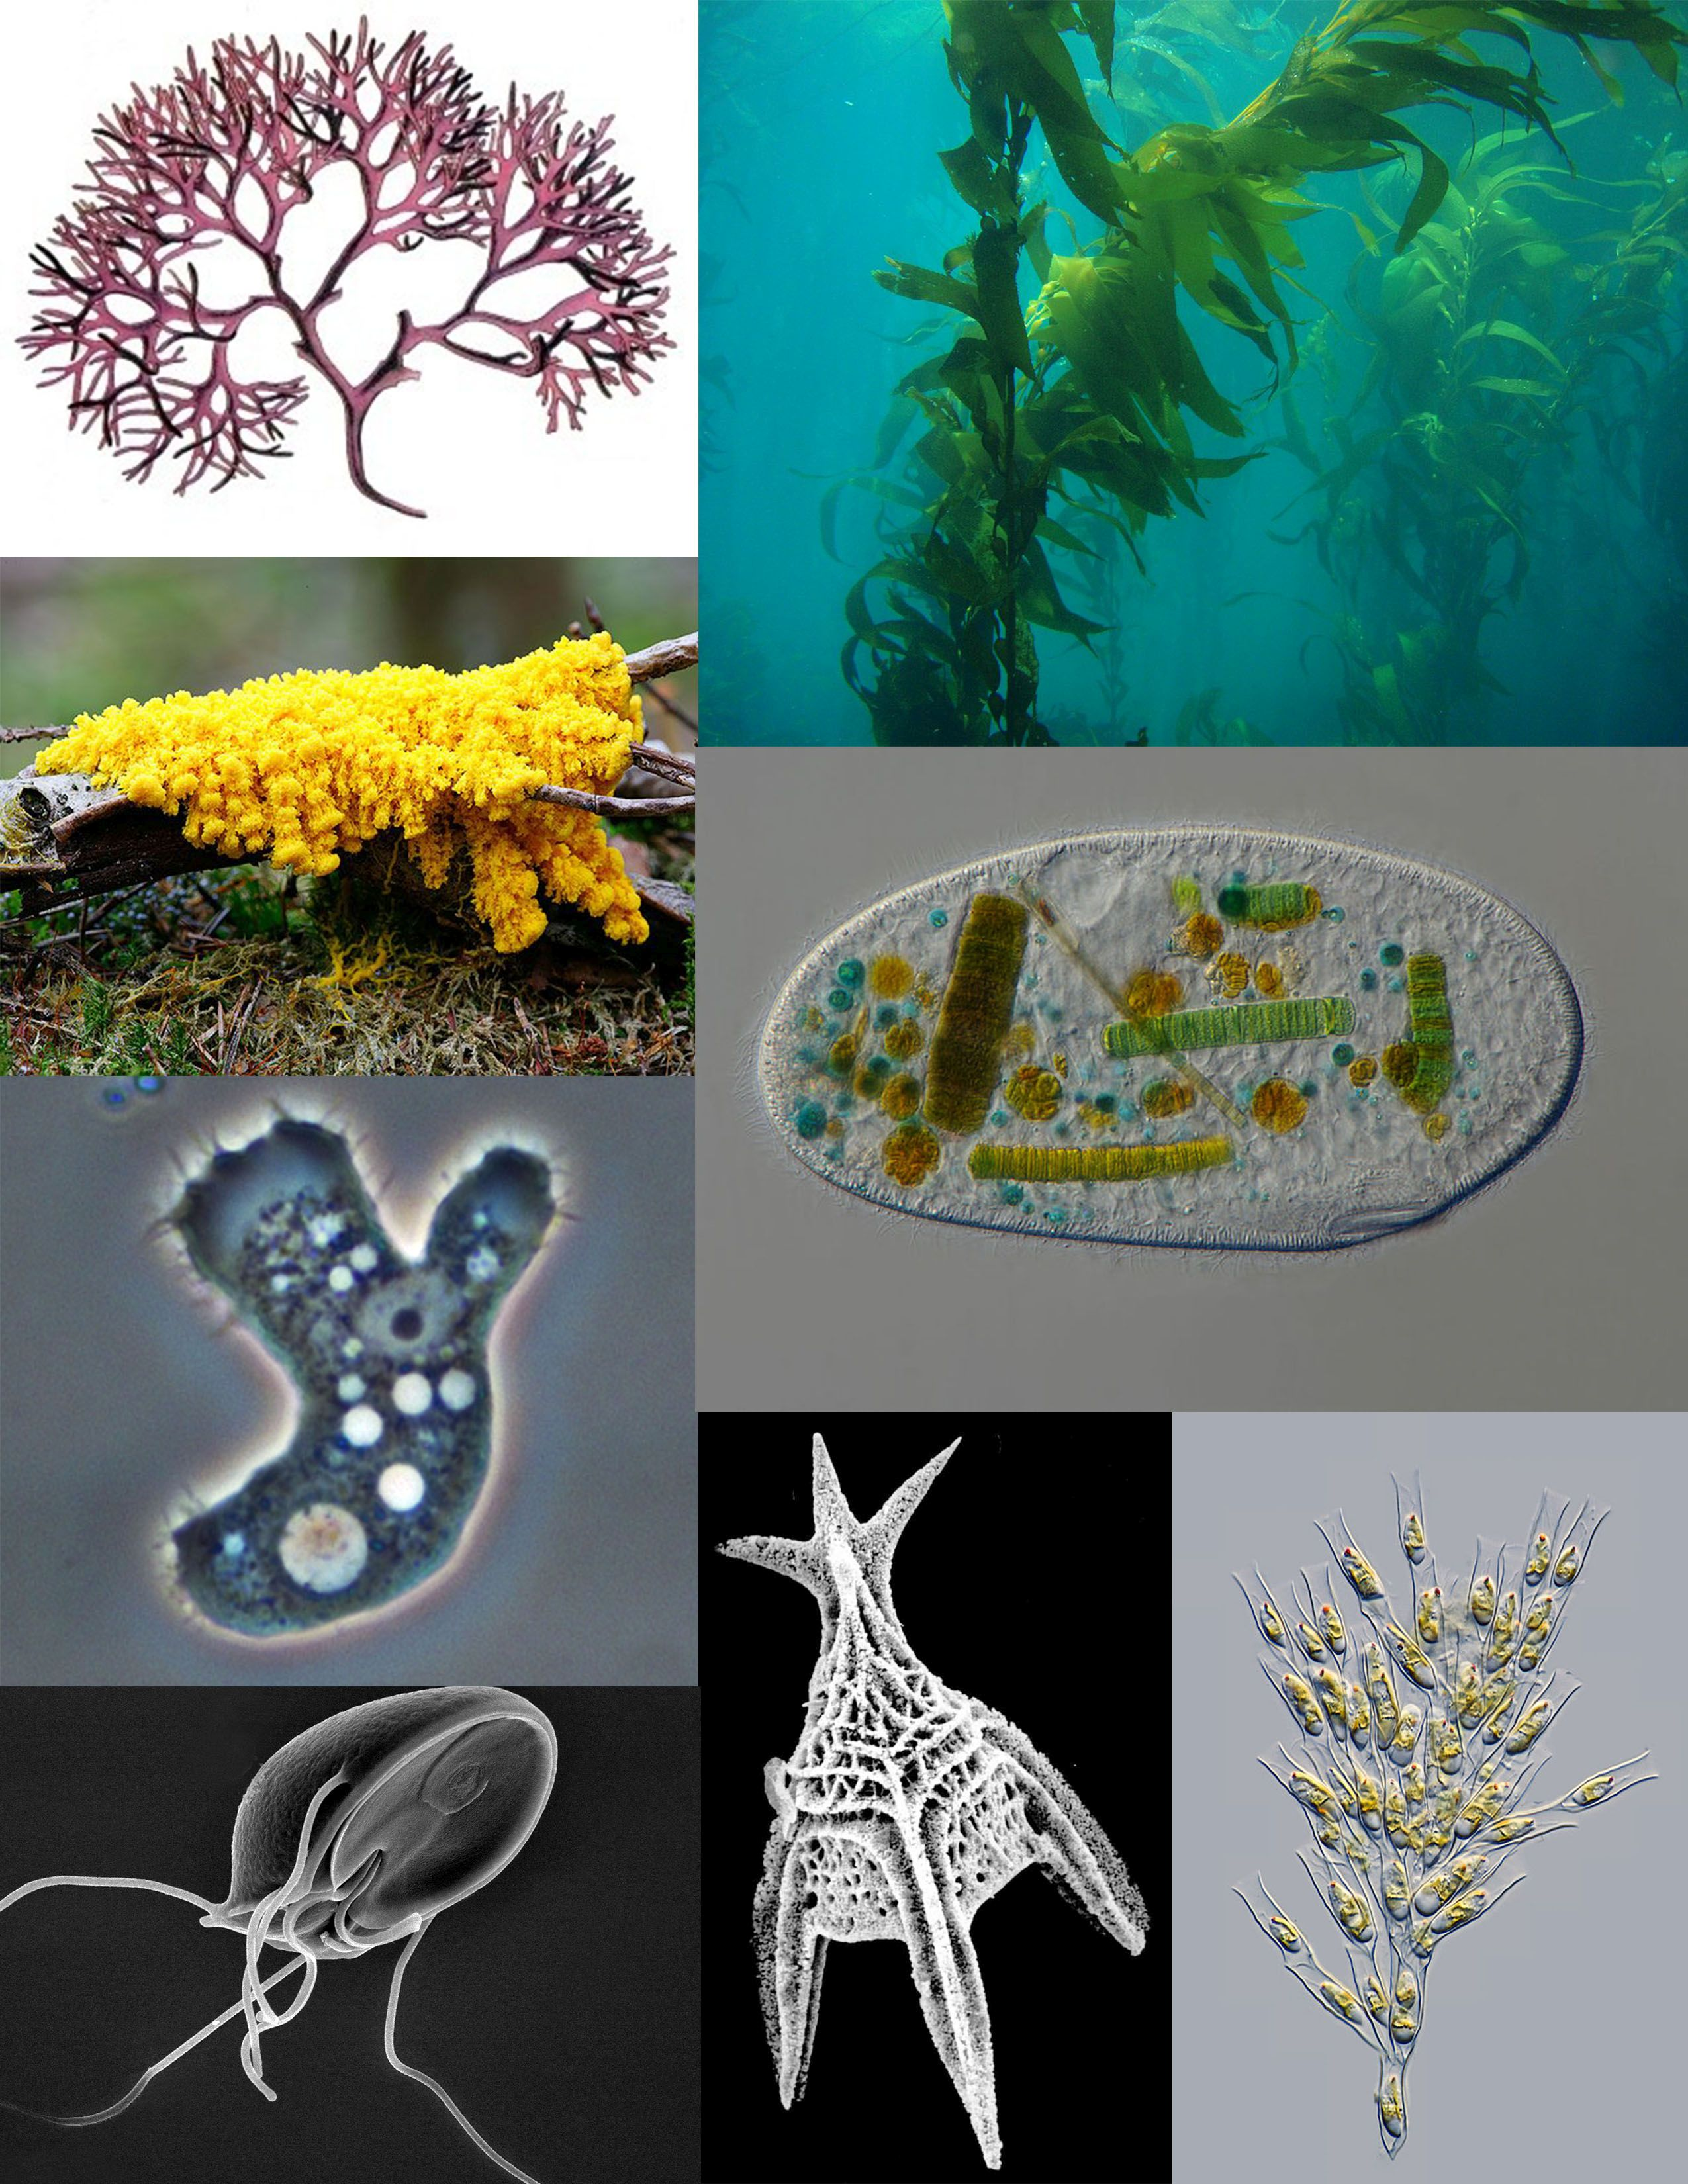
\includegraphics[width=0.7\linewidth]{./figures/protista/Protist_collage_2} 

}

\caption{\href{https://commons.wikimedia.org/wiki/File:Protist_collage_2.jpg}{A sampling of protists:} red algae (Chondrus crispus); brown algae (Giant Kelp); ciliate (Frontonia); golden algae (Dinobryon); Foraminifera (Radiolaria); parasitic flagellate (Giardia muris); pathogenic amoeba (Acanthamoeba); amoebozoan slime mold (Fuligo septica)}\label{fig:protistacollage}
\end{figure}

In antiquity, the two lineages of animals and plants were recognized. They were given the taxonomic rank of Kingdom by the Swedish botanist \href{https://en.wikipedia.org/wiki/Carl_Linnaeus}{Carl Linnaeus}. Though he included the fungi with plants with some reservations, it was later realized that they are quite distinct and warrant a separate kingdom, the composition of which was not entirely clear until the 1980s. The various single-cell eukaryotes were originally placed with plants or animals when they became known. In 1818, the German biologist Georg A. Goldfuss coined the word protozoa to refer to organisms such as ciliates, and this group was expanded until it encompassed all single-celled eukaryotes, and given their own kingdom, the Protista, by \href{https://en.wikipedia.org/wiki/Ernst_Haeckel}{Ernst Haeckel} in 1866.



\begin{figure}

{\centering 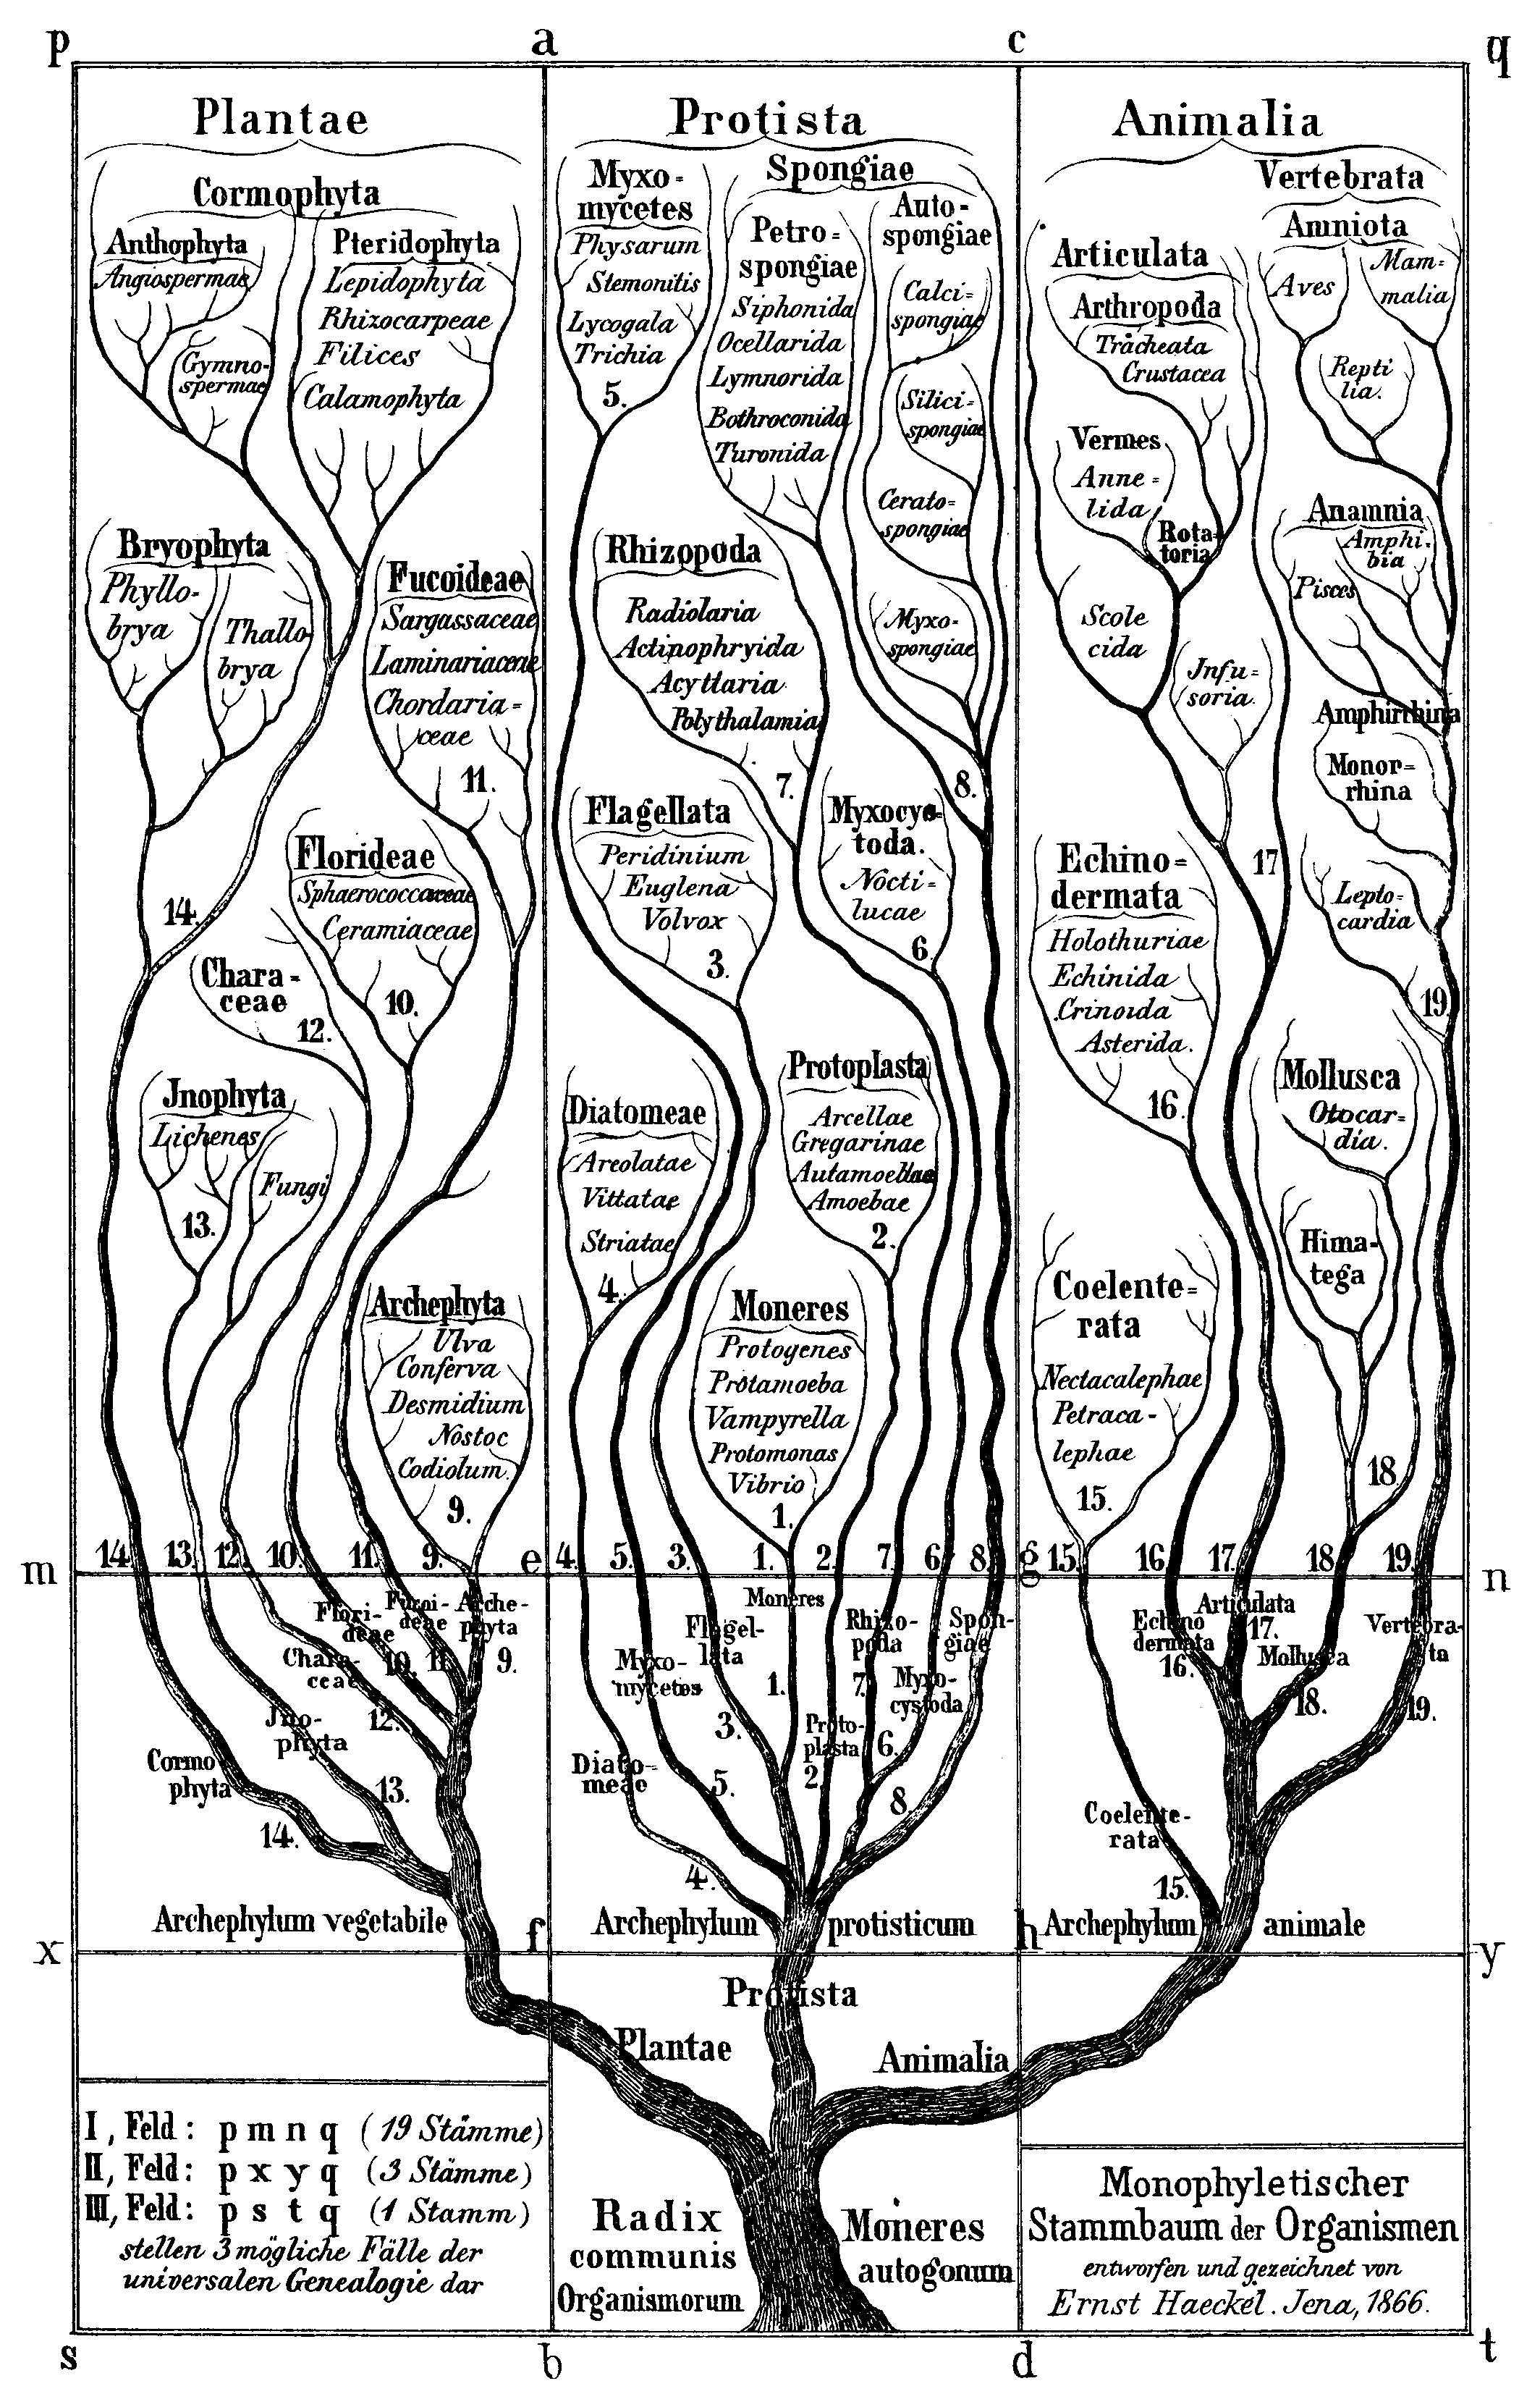
\includegraphics[width=0.7\linewidth]{./figures/protista/Haeckel_arbol_bn} 

}

\caption{\href{https://commons.wikimedia.org/wiki/File:Haeckel_arbol_bn.png}{``Monophyletischer Stambaum der Organismen'' from Generelle Morphologie der Organismen (1866) with the three branches Plantae, Protista, Animalia.}}\label{fig:haeckel3kingdoms}
\end{figure}

The eukaryotes thus came to be composed of four kingdoms:

\begin{itemize}
\tightlist
\item
  Kingdom Protista
\item
  Kingdom Plantae
\item
  Kingdom Fungi
\item
  Kingdom Animalia
\end{itemize}

The protists were understood to be ``primitive forms'', and thus an evolutionary grade, united by their primitive unicellular nature. The disentanglement of the deep splits in the tree of life only really started with DNA sequencing, leading to a system of domains rather than kingdoms as top level rank being put forward by Carl Woese, uniting all the eukaryote kingdoms under the eukaryote domain. At the same time, work on the protist tree intensified, and is still actively going on today. Several alternative classifications have been forwarded, though there is no consensus in the field.

A revised classification in 2012 recognizes five supergroups of eukaryotes as shown in Table \ref{tab:eukaryotetaxonomy}.

\begin{table}[!h]

\caption{\label{tab:eukaryotetaxonomy}A recent (2012) classification of protists.}
\centering
\begin{tabular}[t]{>{\raggedright\arraybackslash}p{8em}>{\raggedright\arraybackslash}p{17em}}
\toprule
Supergroup Name & Organisms\\
\midrule
\rowcolor{gray!6}  Archaeplastida (or Primoplantae) & Land plants, green algae, red algae, and glaucophytes\\
SAR supergroup & Stramenopiles (brown algae, diatoms, etcetera), Alveolata, and Rhizaria (Foraminifera, Radiolaria, and various other amoeboid protozoa)\\
\rowcolor{gray!6}  Excavata & Various flagellate protozoa\\
Amoebozoa & Most lobose amoeboids and slime molds\\
\rowcolor{gray!6}  Opisthokonta & Animals, fungi, choanoflagellates, etcetera\\
\bottomrule
\end{tabular}
\end{table}

The classification of a separate kingdom to the animals and plants was first proposed by John Hogg in 1860 as the kingdom Protoctista; in 1866 Ernst Haeckel also proposed a third kingdom Protista as ``the kingdom of primitive forms''. Originally these also included prokaryotes, but with time these would be removed to a fourth kingdom Monera. In the popular five-kingdom scheme proposed by Robert Whittaker in 1969, the Protista was defined as eukaryotic ``organisms which are unicellular or unicellular-colonial and which form no tissues'', and the fifth kingdom Fungi was established. In the five-kingdom system of Lynn Margulis, the term protist is reserved for microscopic organisms, while the more inclusive kingdom Protoctista (or protoctists) included certain large multicellular eukaryotes, such as kelp, red algae and slime molds. Others use the term protist interchangeably with Margulis's protoctist, to encompass both single-celled and multicellular eukaryotes, including those that form specialized tissues but do not fit into any of the other traditional kingdoms.

Besides their relatively simple levels of organization, protists do not necessarily have much in common. When used, the term ``protists'' is now considered to mean a paraphyletic assemblage of similar-appearing but diverse taxa (biological groups); these taxa do not have an exclusive common ancestor beyond being composed of eukaryotes, and have different life cycles, trophic levels, modes of locomotion and cellular structures. Examples of protists include: amoebas (including nucleariids and Foraminifera); choanaflagellates; ciliates; diatoms; dinoflagellates; Giardia; Plasmodium (which causes malaria); oomycetes (including Phytophthora, the cause of the Great Famine of Ireland); and slime molds. These examples are unicellular, although oomycetes can form filaments, and slime molds can aggregate.

In cladistic systems (classifications based on common ancestry), there are no equivalents to the taxa Protista or Protoctista, as both terms refer to a paraphyletic group that spans the entire eukaryotic tree of life. In cladistic classification, the contents of Protista are mostly distributed among various supergroups: examples include the SAR supergroup (of stramenopiles or heterokonts, alveolates, and Rhizaria); Archaeplastida (or Plantae sensu lato); Excavata (which is mostly unicellular flagellates); and Opisthokonta (which commonly includes unicellular flagellates, but also animals and fungi). ``Protista'', ``Protoctista'', and ``Protozoa'' are therefore considered obsolete. However, the term ``protist'' continues to be used informally as a catch-all term for eukayotic organisms that aren't within other traditional kingdoms. For example, the word ``protist pathogen'' may be used to denote any disease-causing organism that is not plant, animal, fungal, prokaryotic, viral, or subviral.

The term protista was first used by Ernst Haeckel in 1866. Protists were traditionally subdivided into several groups based on similarities to the ``higher'' kingdoms such as:

\begin{itemize}
\tightlist
\item
  Protozoa: unicellular ``animal-like'' (heterotrophic, and sometimes parasitic) organisms that are further sub-divided based on characteristics such as motility, such as the (flagellated) Flagellata, the (ciliated) Ciliophora, the (phagocytic) amoeba, and the (spore-forming) Sporozoa.
\item
  Protophyta: plant-like" (autotrophic) organisms that are composed mostly of unicellular algae. The dinoflagelates, diatoms and Euglena-like flagellates are photosynthetic protists.
\item
  Molds: ``Mold'' generally refer to fungi; but slime molds and water molds are fungus-like" (saprophytic) protists, although some are pathogens.
\end{itemize}

Some protists, sometimes called ambiregnal protists, have been considered to be both protozoa and algae or fungi (e.g., slime molds and flagellated algae). Conflicts, such as these -- for example the dual-classification of Euglenids and Dinobryons, which are mixotrophic -- is an example of why the kingdom Protista was adopted.

These traditional subdivisions, largely based on superficial commonalities, have been replaced by classifications based on phylogenetics (evolutionary relatedness among organisms). Molecular analyses in modern taxonomy have been used to redistribute former members of this group into diverse and sometimes distantly related phyla. For instance, the water molds are now considered to be closely related to photosynthetic organisms such as Brown algae and Diatoms, the slime molds are grouped mainly under Amoebozoa, and the Amoebozoa itself includes only a subset of the ``Amoeba'' group, and significant number of erstwhile ``Amoeboid'' genera are distributed among Rhizarians and other Phyla.

However, the older terms are still used as informal names to describe the morphology and ecology of various protists. For example, the term protozoa is used to refer to heterotrophic species of protists that do not form filaments.

Systematists today do not treat Protista as a formal taxon, but the term ``protist'' is still commonly used for convenience in two ways. The most popular contemporary definition is a phylogenetic one, that identifies a paraphyletic group: a protist is any eukaryote that is not an animal, (land) plant, or (true) fungus; this definition excludes many unicellular groups, like the Microsporidia (fungi), many Chytridiomycetes (fungi), and yeasts (fungi), and also a non-unicellular group included in Protista in the past, the Myxozoa (animal).

The taxonomy of protists is still changing. Newer classifications attempt to present monophyletic groups based on morphological (especially ultrastructural), biochemical (chemotaxonomy) and DNA sequence (molecular research) information. Because the protists as a whole are paraphyletic, new systems often split up or abandon the kingdom, instead treating the protist groups as separate lines of eukaryotes.

\onecolumn
\begin{sidewaystable}[!h]
\caption{\label{tab:protistmetabo}Nutritional types in protist metabolism}
\centering
\begin{tabular}[t]{>{\raggedright\arraybackslash}p{10em}>{\raggedright\arraybackslash}p{20em}>{\raggedright\arraybackslash}p{15em}>{\raggedright\arraybackslash}p{20em}}
\toprule
Nutritional Type & Source of Energy & Source of Carbon & Examples\\
\midrule
\rowcolor{gray!6}   Photoautotrophs  &  Sunlight  &  Organic compounds or carbon fixation &  Most algae \\
 Chemoheterotrophs &  Organic compounds  &  Organic compounds  &  Apicomplexa, Trypanosomes or Amoebae \\
\bottomrule
\end{tabular}
\end{sidewaystable}

\twocolumn

\hypertarget{protozoa}{%
\section{Protozoa}\label{protozoa}}

\href{https://en.wikipedia.org/wiki/Protozoa}{Protozoa} (also protozoan, plural protozoans) is an informal term for a group of single-celled eukaryotes, either free-living or parasitic, which feed on organic matter such as other microorganisms or organic tissues and debris. Historically, protozoans were regarded as ``one-celled animals'', because they often possess animal-like behaviours, such as motility and predation, and lack a cell wall, as found in plants and many algae. Although the traditional practice of grouping protozoa with animals is no longer considered valid, the term continues to be used in a loose way to describe single-celled protists (that is, eukaryotes that aren't animals, plants, or fungi) that feed by heterotrophy.

In some systems of biological classification, Protozoa remains a high-level taxonomic group. When first introduced by Georg Goldfuss in 1818, Protozoa was erected as a class within the animals, and its etymology is literally ``first animals''. In later classification schemes it was elevated to a variety of higher ranks, including phylum, subkingdom and kingdom, and sometimes included within Protoctista or Protista. With the advent of techniques such as molecular phylogenetics, it was realized that Protozoa did not represent a natural group; but while it is not an accepted taxon in cladistic analyses, some systematists continue to use it as a formal taxon.

In a series of classifications proposed by Thomas Cavalier-Smith and his collaborators since 1981, Protozoa has been ranked as a kingdom. The seven-kingdom scheme presented by Ruggiero et al.~in 2015, places eight phyla under Kingdom Protozoa: Euglenozoa, Amoebozoa, Metamonada, Choanozoa sensu Cavalier-Smith, Loukozoa, Percolozoa, Microsporidia and Sulcozoa. Notably, this kingdom excludes several major groups of organisms traditionally placed among the protozoa, including the ciliates, dinoflagellates, foraminifera, and the parasitic apicomplexans, all of which are classified under Kingdom Chromista. Kingdom Protozoa, as defined in this scheme, does not form a natural group or clade, but a paraphyletic group or evolutionary grade, within which the members of Fungi, Animalia and Chromista are thought to have evolved.

The word ``protozoa'' (singular protozoon or protozoan) was coined in 1818 by zoologist Georg August Goldfuss, as the Greek equivalent of the German Urthiere, meaning ``primitive, or original animals'' (ur- `proto-' + Thier `animal'). Goldfuss created Protozoa as a class containing what he believed to be the simplest animals. Originally, the group included not only single-celled microorganisms but also some ``lower'' multicellular animals, such as rotifers, corals, sponges, jellyfish, bryozoa and polychaete worms. The term Protozoa is formed from the Greek words πρῶτος (prôtos), meaning ``first'', and ζῶα (zôa), plural of ζῶον (zôon), meaning ``animal''. The use of Protozoa as a formal taxon has been discouraged by some researchers, mainly because the term implies kinship with animals (Metazoa) and promotes an arbitrary separation of ``animal-like'' from ``plant-like'' organisms.

In 1848, as a result of advancements in cell theory pioneered by Theodor Schwann and Matthias Schleiden, the anatomist and zoologist C. T. von Siebold proposed that the bodies of protozoans such as ciliates and amoebae consisted of single cells, similar to those from which the multicellular tissues of plants and animals were constructed. Von Siebold redefined Protozoa to include only such unicellular forms, to the exclusion of all metazoa (animals). At the same time, he raised the group to the level of a phylum containing two broad classes of microorganisms: Infusoria (mostly ciliates and flagellated algae), and Rhizopoda (amoeboid organisms). The definition of Protozoa as a phylum or sub-kingdom composed of ``unicellular animals'' was adopted by the zoologist Otto Bütschli---celebrated at his centenary as the ``architect of protozoology''---and the term came into wide use.

As a phylum under Animalia, the Protozoa were firmly rooted in the old ``two-kingdom'' classification of life, according to which all living beings were classified as either animals or plants. As long as this scheme remained dominant, the protozoa were understood to be animals and studied in departments of Zoology, while photosynthetic microorganisms and microscopic fungi---the so-called Protophyta---were assigned to the Plants, and studied in departments of Botany.

Criticism of this system began in the latter half of the 19th century, with the realization that many organisms met the criteria for inclusion among both plants and animals. For example, the algae Euglena and Dinobryon have chloroplasts for photosynthesis, but can also feed on organic matter and are motile. In 1860, John Hogg argued against the use of ``protozoa'', on the grounds that ``naturalists are divided in opinion---and probably some will ever continue so---whether many of these organisms, or living beings, are animals or plants.'' As an alternative, he proposed a new kingdom called Primigenum, consisting of both the protozoa and unicellular algae (protophyta), which he combined together under the name ``Protoctista''. In Hoggs's conception, the animal and plant kingdoms were likened to two great ``pyramids'' blending at their bases in the Kingdom Primigenum.

Six years later, Ernst Haeckel also proposed a third kingdom of life, which he named Protista. At first, Haeckel included a few multicellular organisms in this kingdom, but in later work he restricted the Protista to single-celled organisms, or simple colonies whose individual cells are not differentiated into different kinds of tissues.

Despite these proposals, Protozoa emerged as the preferred taxonomic placement for heterotrophic microorganisms such as amoebae and ciliates, and remained so for more than a century. In the course of the 20th century, however, the old ``two kingdom'' system began to weaken, with the growing awareness that fungi did not belong among the plants, and that most of the unicellular protozoa were no more closely related to the animals than they were to the plants. By mid-century, some biologists, such as Herbert Copeland, Robert H. Whittaker and Lynn Margulis, advocated the revival of Haeckel's Protista or Hogg's Protoctista as a kingdom-level eukaryotic group, alongside Plants, Animals and Fungi. A variety of multi-kingdom systems were proposed, and Kingdoms Protista and Protoctista became well established in biology texts and curricula.

While many taxonomists have abandoned Protozoa as a high-level group, Thomas Cavalier-Smith has retained it as a kingdom in the various classifications he has proposed. As of 2015, Cavalier-Smith's Protozoa excludes several major groups of organisms traditionally placed among the protozoa, including the ciliates, dinoflagellates and foraminifera (all members of the SAR supergroup). In its current form, his kingdom Protozoa is a paraphyletic group which includes a common ancestor and most of its descendants, but excludes two important clades that branch within it: the animals and fungi.

Since the protozoa, as traditionally defined, can no longer be regarded as ``primitive animals'' the terms ``protists'', ``Protista'' or ``Protoctista'' are sometimes preferred. In 2005, members of the Society of Protozoologists voted to change its name to the International Society of Protistologists.
Free-living protozoans are common and often abundant in fresh, brackish and salt water, as well as other moist environments, such as soils and mosses. Some species thrive in extreme environments such as hot springs and hypersaline lakes and lagoons. All protozoa require a moist habitat; however, some can survive for long periods of time in dry environments, by forming resting cysts which enable them to remain dormant until conditions improve.

Parasitic and symbiotic protozoa live on or within other organisms, including vertebrates and invertebrates, as well as plants and other single-celled organisms. Some are harmless or beneficial to their host organisms; others may be significant causes of diseases, such as babesia, malaria and toxoplasmosis.

Association between protozoan symbionts and their host organisms can be mutually beneficial. Flagellated protozoans such as Trichonympha and Pyrsonympha inhabit the guts of termites, where they enable their insect host to digest wood by helping to break down complex sugars into smaller, more easily digested molecules. A wide range of protozoans live commensally in the rumens of ruminant animals, such as cattle and sheep. These include flagellates, such as Trichomonas, and ciliated protozoa, such as Isotricha and Entodinium. The ciliate subclass Astomatia is composed entirely of mouthless symbionts adapted for life in the guts of annelid worms.

All protozoans are heterotrophic, deriving nutrients from other organisms, either by ingesting them whole or consuming their organic remains and waste-products. Some protozoans take in food by phagocytosis, engulfing organic particles with pseudopodia (as amoebae do), or taking in food through a specialized mouth-like aperture called a cytostome. Others take in food by osmotrophy, absorbing dissolved nutrients through their cell membranes.

Parasitic protozoans use a wide variety of feeding strategies, and some may change methods of feeding in different phases of their life cycle. For instance, the malaria parasite Plasmodium feeds by pinocytosis during its immature trophozoite stage of life (ring phase), but develops a dedicated feeding organelle (cytostome) as it matures within a host's red blood cell.

Protozoa may also live as mixotrophs, supplementing a heterotrophic diet with some form of autotrophy. Some protozoa form close associations with symbiotic photosynthetic algae, which live and grow within the membranes of the larger cell and provide nutrients to the host. Others practice kleptoplasty, stealing chloroplasts from prey organisms and maintaining them within their own cell bodies as they continue to produce nutrients through photosynthesis. The ciliate Mesodinium rubrum retains functioning plastids from the cryptophyte algae on which it feeds, using them to nourish themselves by autotrophy. These, in turn, may be passed along to dinoflagellates of the genus Dinophysis, which prey on Mesodinium rubrum but keep the enslaved plastids for themselves. Within Dinophysis, these plastids can continue to function for months.

Organisms traditionally classified as protozoa are abundant in aqueous environments and soil, occupying a range of trophic levels. The group includes flagellates (which move with the help of whip-like structures called flagella), ciliates (which move by using hair-like structures called cilia) and amoebae (which move by the use of foot-like structures called pseudopodia). Some protozoa are sessile, and do not move at all.

Unlike plants, fungi and most types of algae, protozoans do not typically have a rigid cell wall, but are usually enveloped by elastic structures of membranes that permit movement of the cell. In some protozoans, such as the ciliates and euglenozoans, the cell is supported by a composite membranous envelope called the ``pellicle''. The pellicle gives some shape to the cell, especially during locomotion. Pellicles of protozoan organisms vary from flexible and elastic to fairly rigid. In ciliates and Apicomplexa, the pellicle is supported by closely packed vesicles called alveoli. In euglenids, it is formed from protein strips arranged spirally along the length of the body. Familiar examples of protists with a pellicle are the euglenoids and the ciliate Paramecium. In some protozoa, the pellicle hosts epibiotic bacteria that adhere to the surface by their fimbriae (attachment pili).

Some protozoa have two-phase life cycles, alternating between proliferative stages (e.g., trophozoites) and dormant cysts. As cysts, protozoa can survive harsh conditions, such as exposure to extreme temperatures or harmful chemicals, or long periods without access to nutrients, water, or oxygen for periods of time. Being a cyst enables parasitic species to survive outside of a host, and allows their transmission from one host to another. When protozoa are in the form of trophozoites (Greek tropho = to nourish), they actively feed. The conversion of a trophozoite to cyst form is known as encystation, while the process of transforming back into a trophozoite is known as excystation.

Protozoans reproduce asexually by binary fission or multiple fission. Many protozoan species also exchange genetic material by sexual means (typically, through conjugation), but this is generally decoupled from the process of reproduction, and does not immediately result in increased population.

Although meiotic sex is widespread among present day eukaryotes, it has, until recently, been unclear whether or not eukaryotes were sexual early in their evolution. Due to recent advances in gene detection and other techniques, evidence has been found for some form of meiotic sex in an increasing number of protozoans of ancient lineage that diverged early in eukaryotic evolution. (See eukaryote reproduction.) Thus, such findings suggest that meiotic sex arose early in eukaryotic evolution. Examples of protozoan meiotic sexuality are described in the articles Amoebozoa, Giardia lamblia, Leishmania, Plasmodium falciparum biology, Paramecium, Toxoplasma gondii, Trichomonas vaginalis and Trypanosoma brucei.

Historically, the Protozoa were classified as ``unicellular animals'', as distinct from the Protophyta, single-celled photosynthetic organisms (algae) which were considered primitive plants. Both groups were commonly given the rank of phylum, under the kingdom Protista. In older systems of classification, the phylum Protozoa was commonly divided into several sub-groups, reflecting the means of locomotion. Classification schemes differed, but throughout much of the 20th century the major groups of Protozoa included:

\begin{itemize}
\tightlist
\item
  Flagellates, or Mastigophora (motile cells equipped with whiplike organelles of locomotion, e.g., Giardia lamblia)
\item
  Amoebae or Sarcodina (cells that move by extending pseudopodia or lamellipodia, e.g., Entamoeba histolytica)
\item
  Sporozoans, or Sporozoa (parasitic, spore-producing cells, whose adult form lacks organs of motility, e.g., Plasmodium knowlesi)

  \begin{itemize}
  \tightlist
  \item
    Apicomplexa (now in Alveolata)
  \item
    Microsporidia (now in Fungi)
  \item
    Ascetosporea (now in Rhizaria)
  \item
    Myxosporidia (now in Cnidaria)
  \end{itemize}
\item
  Ciliates, or Ciliophora (cells equipped with large numbers of short hairlike organs of locomotion, e.g.~Balantidium coli)
\end{itemize}



\begin{figure}

{\centering 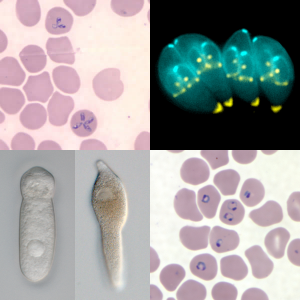
\includegraphics[width=0.7\linewidth]{./figures/protista/Apicomplexa_Composite_Image} 

}

\caption{\href{https://commons.wikimedia.org/wiki/File:Apicomplexa_Composite_Image.png}{Composite image} of various Apicomplexan parasites showing Babesia microti in red blood cells (top left), toxoplasma gondii (top right), a septate eugregarine (bottom left), Lankesteria cystodytae (bottom middle), and Plasmodium falciparum in red blood cells (bottom right).}\label{fig:apicomplexa}
\end{figure}

With the emergence of molecular phylogenetics and tools enabling researchers to directly compare the DNA of different organisms, it became evident that, of the main sub-groups of Protozoa, only the ciliates (Ciliophora) formed a natural group, or monophyletic clade (that is, a distinct lineage of organisms sharing common ancestry). The other classes or subphyla of Protozoa were all polyphyletic groups composed of organisms that, despite similarities of appearance or way of life, were not necessarily closely related to one another. In the system of eukaryote classification currently endorsed by the International Society of Protistologists, members of the old phylum Protozoa have been distributed among a variety of supergroups.

A number of protozoan pathogens are human parasites, causing diseases such as malaria (by Plasmodium), amoebiasis, giardiasis, toxoplasmosis, cryptosporidiosis, trichomoniasis, Chagas disease, leishmaniasis, African trypanosomiasis (sleeping sickness), Acanthamoeba keratitis, and primary amoebic meningoencephalitis (naegleriasis).

The protozoan Ophryocystis elektroscirrha is a parasite of butterfly larvae, passed from female to caterpillar. Severely infected individuals are weak, unable to expand their wings, or unable to eclose, and have shortened lifespans, but parasite levels vary in populations. Infection creates a culling effect, whereby infected migrating animals are less likely to complete the migration. This results in populations with lower parasite loads at the end of the migration. This is not the case in laboratory or commercial rearing, where after a few generations, all individuals can be infected

\hypertarget{flagellates}{%
\section{Flagellates}\label{flagellates}}

In older classifications, flagellated protozoa were grouped in Flagellata (= Mastigophora), sometimes divided in Phytoflagellata (= Phytomastigina, mostly autotrophic) and Zooflagellata (= Zoomastigina, heterotrophic). They were sometimes grouped with Sarcodina (ameboids) in the group Sarcomastigophora.

Excavata is a major supergroup of unicellular organisms eukayotes that are classified based on their flagellar structures, and they are considered to be the most basal Flagellate lineage. It contains a variety of free-living and symbiotic forms, and also includes some important parasites of humans, including Giardia and Trichomonas. Except for Euglenozoa, they are all non-photosynthetic.

Euglena is a genus of single cell flagellate eukaryotes. It is the best known and most widely studied member of the class Euglenoidea, a diverse group containing some 54 genera and at least 800 species. Species of Euglena are found in freshwater and salt water. They are often abundant in quiet inland waters where they may bloom in numbers sufficient to color the surface of ponds and ditches green (E. viridis) or red (E. sanguinea).

\begin{figure}

{\centering 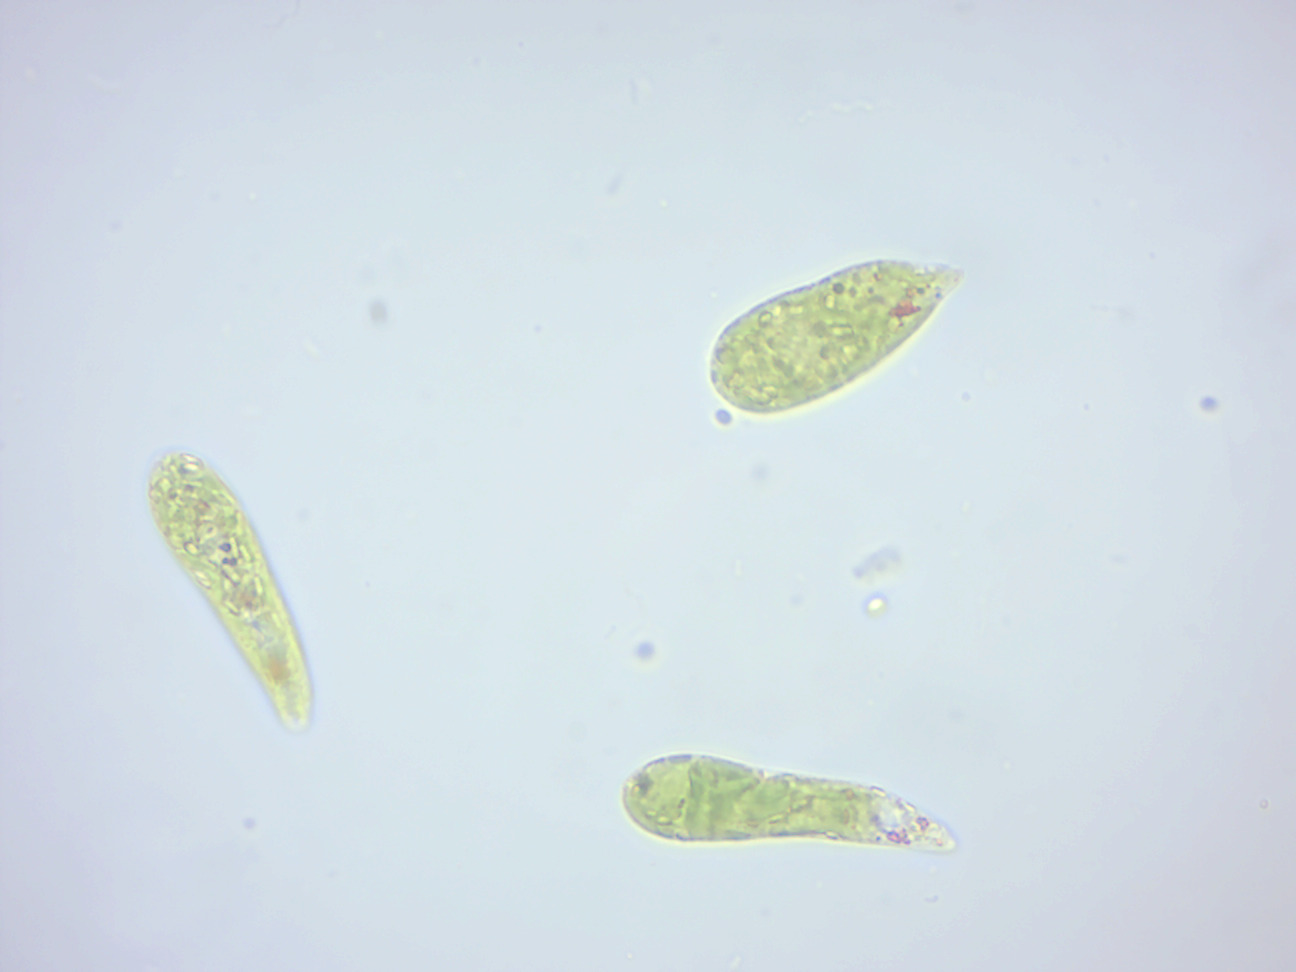
\includegraphics[width=0.7\linewidth]{./figures/protista/euglena} 

}

\caption{Euglena.}\label{fig:euglena}
\end{figure}

The species Euglena gracilis has been used extensively in the laboratory as a model organism.

Most species of Euglena have photosynthesizing chloroplasts within the body of the cell, which enable them to feed by autotrophy, like plants. However, they can also take nourishment heterotrophically, like animals. Since Euglena have features of both animals and plants, early taxonomists, working within the Linnaean two-kingdom system of biological classification, found them difficult to classify. It was the question of where to put such ``unclassifiable'' creatures that prompted Ernst Haeckel to add a third living kingdom (a fourth kingdom in toto) to the Animale, Vegetabile (and Lapideum meaning Mineral) of Linnaeus: the Kingdom Protista.

When feeding as a heterotroph, Euglena takes in nutrients by osmotrophy, and can survive without light on a diet of organic matter, such as beef extract, peptone, acetate, ethanol or carbohydrates. When there is sufficient sunlight for it to feed by phototrophy, it uses chloroplasts containing the pigments chlorophyll a and chlorophyll b to produce sugars by photosynthesis. Euglena's chloroplasts are surrounded by three membranes, while those of plants and the green algae (among which earlier taxonomists often placed Euglena) have only two membranes. This fact has been taken as morphological evidence that Euglena's chloroplasts evolved from a eukaryotic green alga. Thus, the similarities between Euglena and plants would have arisen not because of kinship but because of a secondary endosymbiosis. Molecular phylogenetic analysis has lent support to this hypothesis, and it is now generally accepted.

Euglena chloroplasts contain pyrenoids, used in the synthesis of paramylon, a form of starch energy storage enabling Euglena to survive periods of light deprivation. The presence of pyrenoids is used as an identifying feature of the genus, separating it from other euglenoids, such as Lepocinclis and Phacus.

Euglena have two flagella rooted in basal bodies located in a small reservoir at the front of the cell. Typically, one flagellum is very short, and does not protrude from the cell, while the other is long enough to be seen with light microscopy. In some species, such as Euglena mutabilis, both flagella are ``non-emergent''--entirely confined to the interior of the cell's reservoir--and consequently cannot be seen in the light microscope. In species that possess a long, emergent flagellum, it may be used to help the organism swim. The surface of the flagellum is coated with about 30,000 extremely fine filaments called mastigonemes.

Like other euglenoids, Euglena possess a red eyespot, an organelle composed of carotenoid pigment granules. The red spot itself is not thought to be photosensitive. Rather, it filters the sunlight that falls on a light-detecting structure at the base of the flagellum (a swelling, known as the paraflagellar body), allowing only certain wavelengths of light to reach it. As the cell rotates with respect to the light source, the eyespot partially blocks the source, permitting the Euglena to find the light and move toward it (a process known as phototaxis).

Euglena lacks a cell wall. Instead, it has a pellicle made up of a protein layer supported by a substructure of microtubules, arranged in strips spiraling around the cell. The action of these pellicle strips sliding over one another, known as metaboly, gives Euglena its exceptional flexibility and contractility. The mechanism of this euglenoid movement is not understood, but its molecular basis may be similar to that of amoeboid movement.

In low moisture conditions, or when food is scarce, Euglena forms a protective wall around itself and lies dormant as a resting cyst until environmental

Euglena reproduce asexually through binary fission, a form of cell division. Reproduction begins with the mitosis of the cell nucleus, followed by the division of the cell itself. Euglena divide longitudinally, beginning at the front end of the cell, with the duplication of flagellar processes, gullet and stigma. Presently, a cleavage forms in the anterior, and a V-shaped bifurcation gradually moves toward the posterior, until the two halves are entirely separated

\hypertarget{ciliates}{%
\section{Ciliates}\label{ciliates}}

The ciliates are a group of protozoans characterized by the presence of hair-like organelles called cilia, which are identical in structure to eukaryotic flagella, but are in general shorter and present in much larger numbers, with a different undulating pattern than flagella. Cilia occur in all members of the group (although the peculiar Suctoria only have them for part of their life-cycle) and are variously used in swimming, crawling, attachment, feeding, and sensation.



\begin{figure}

{\centering 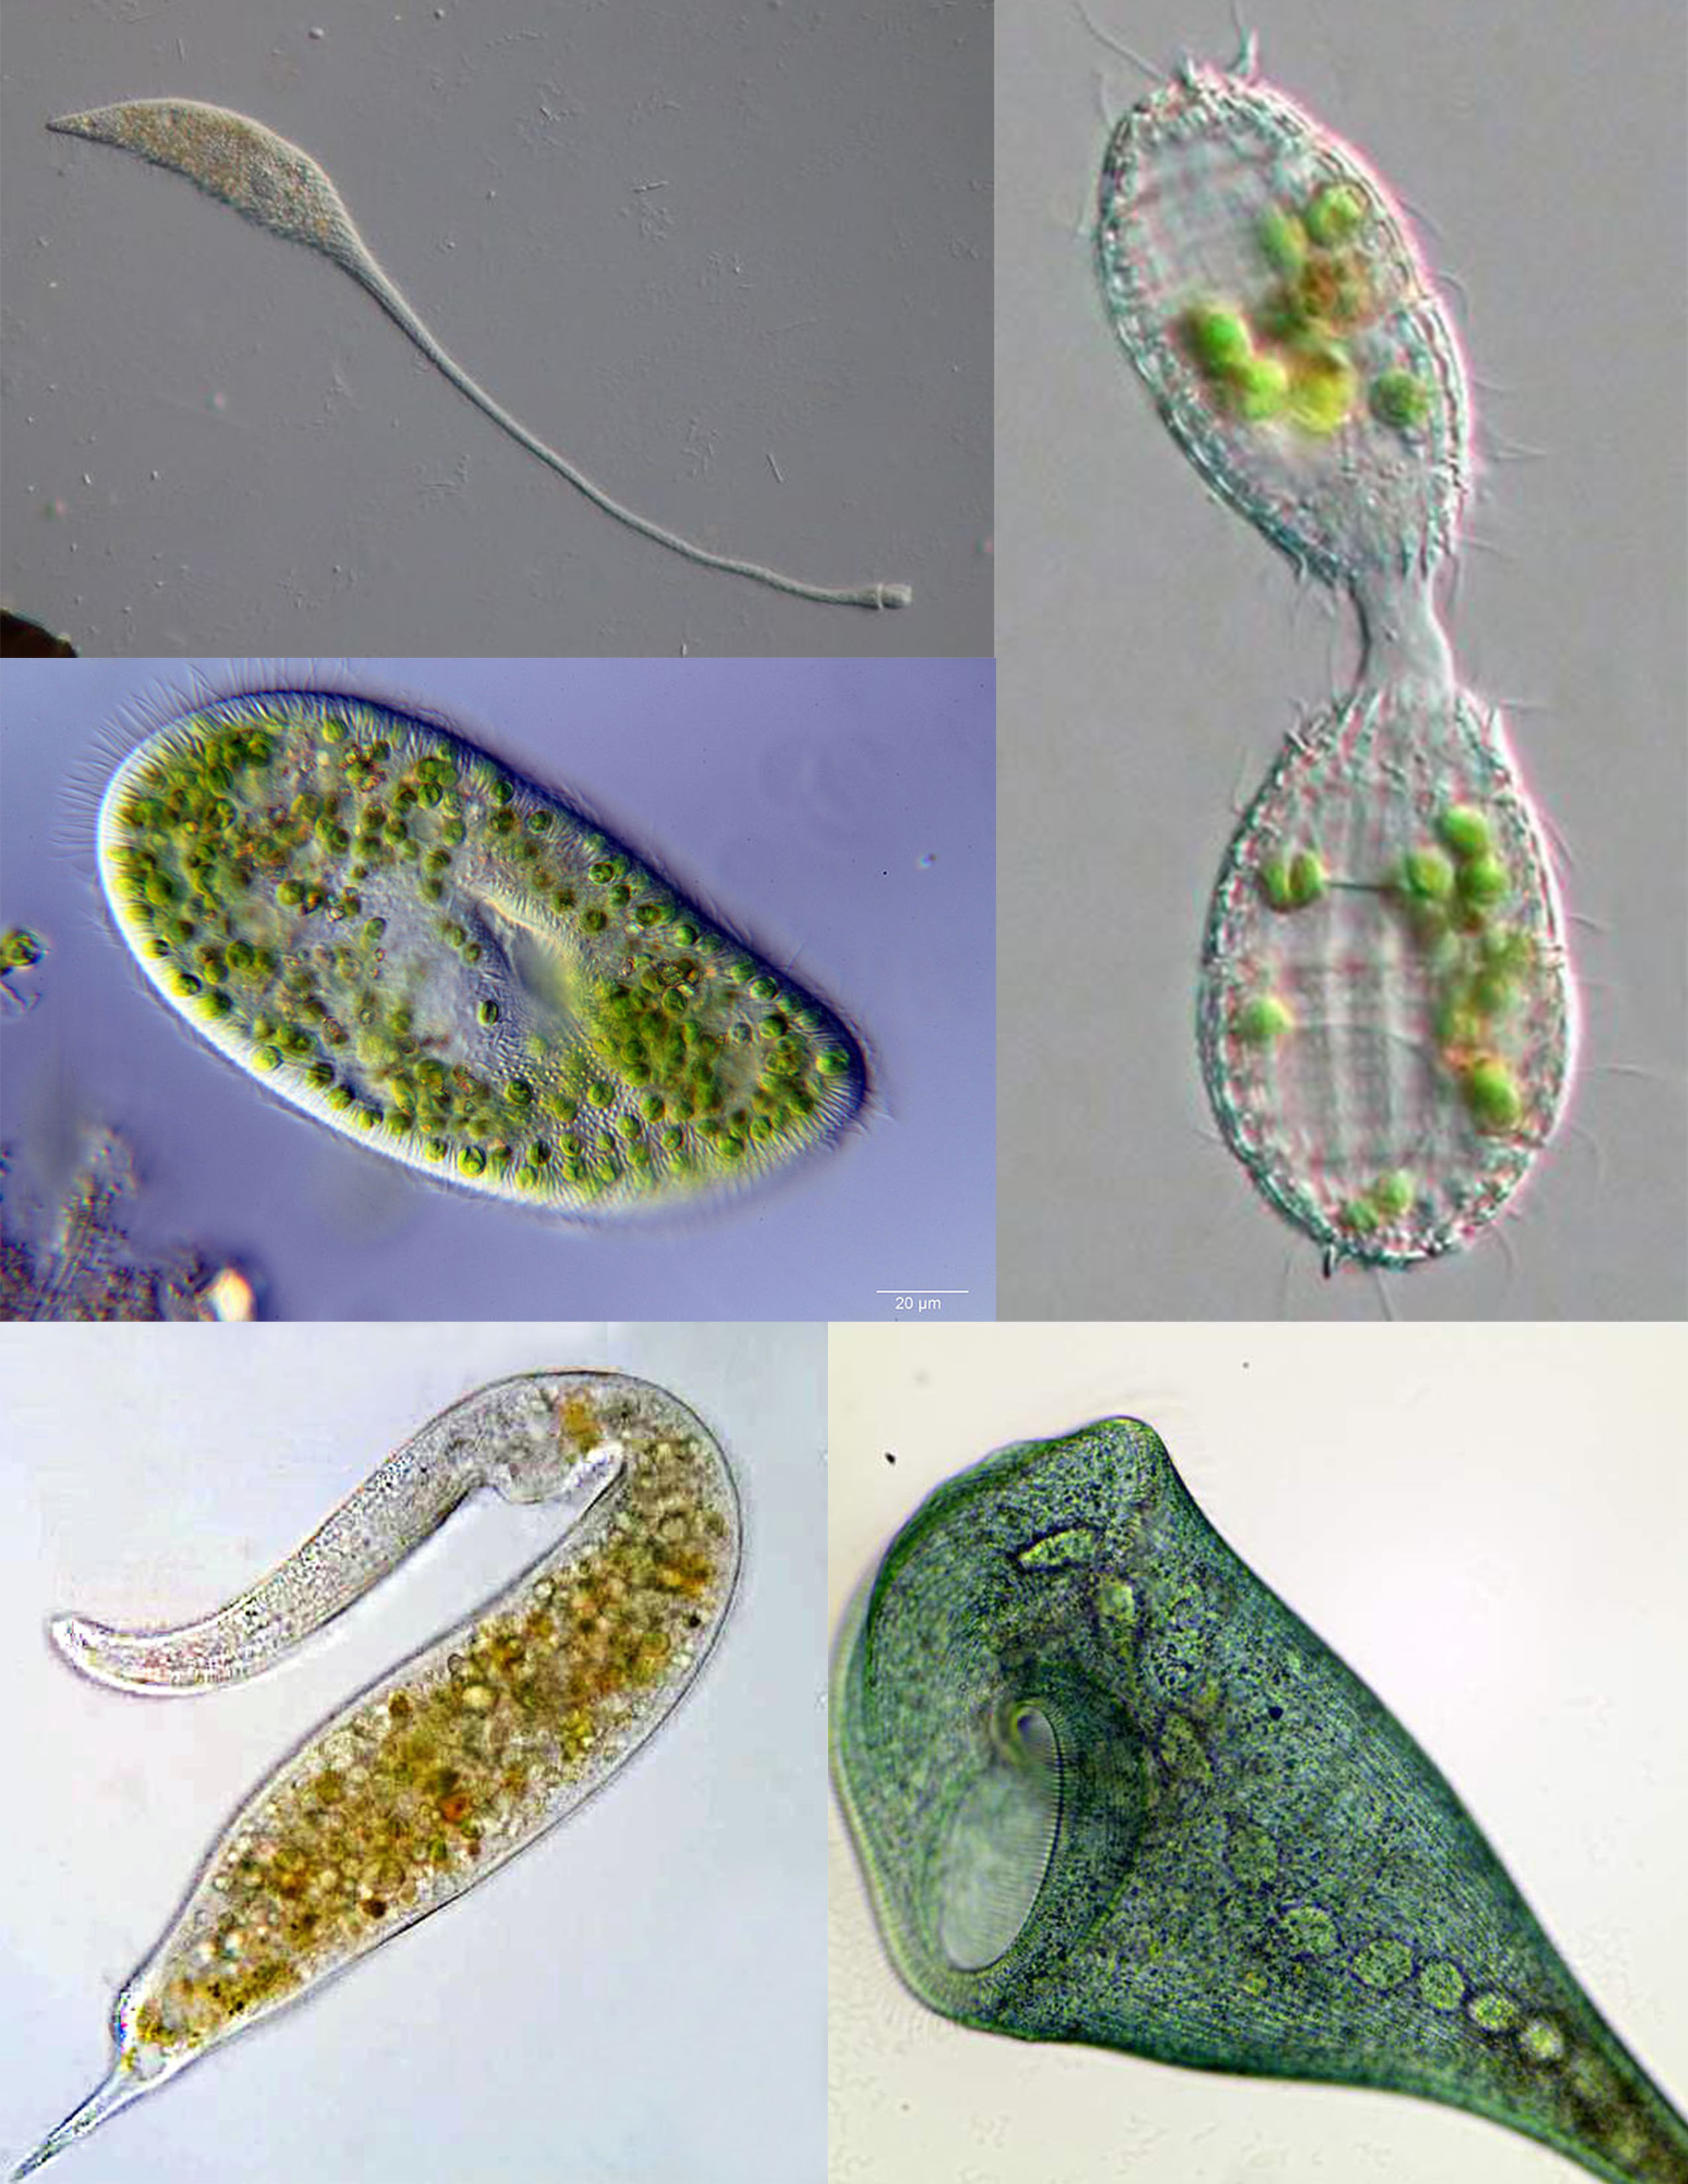
\includegraphics[width=0.7\linewidth]{./figures/protista/Ciliate_collage} 

}

\caption{\href{https://commons.wikimedia.org/wiki/File:Ciliate_collage.jpg}{Composite image} of various ciliates: Lacrymaria olor, Paramecium bursaria, Coleps, Dileptus, Stentor coeruleus.}\label{fig:ciliata}
\end{figure}

Ciliates are an important group of protists, common almost anywhere there is water --- in lakes, ponds, oceans, rivers, and soils. About 4,500 unique free-living species have been described, and the potential number of extant species is estimated at 27,000--40,000. Included in this number are many ectosymbiotic and endosymbiotic species, as well as some obligate and opportunistic parasites. Ciliate species range in size from as little as 10 µm in some colpodeans to as much as 4 mm in length in some geleiids, and include some of the most morphologically complex protozoans.

Unlike most other eukaryotes, ciliates have two different sorts of nuclei: a tiny, diploid micronucleus (the ``generative nucleus,'' which carries the germline of the cell), and a large, polyploid macronucleus (the ``vegetative nucleus,'' which takes care of general cell regulation, expressing the phenotype of the organism). The latter is generated from the micronucleus by amplification of the genome and heavy editing. The micronucleus passes its genetic material to offspring, but does not express its genes. The macronucleus provides the small nuclear RNA for vegetative growth.

Division of the macronucleus occurs by amitosis, and the segregation of the chromosomes occurs by a process whose mechanism is unknown. This process is not perfect, and after about 200 generations the cell shows signs of aging. Periodically the macronuclei must be regenerated from the micronuclei. In most, this occurs during conjugation. Here two cells line up, the micronuclei undergo meiosis, some of the haploid daughters are exchanged and then fuse to form new micronuclei and macronuclei.

Food vacuoles are formed through phagocytosis and typically follow a particular path through the cell as their contents are digested and broken down by lysosomes so the substances the vacuole contains are then small enough to diffuse through the membrane of the food vacuole into the cell. Anything left in the food vacuole by the time it reaches the cytoproct (anal pore) is discharged by exocytosis. Most ciliates also have one or more prominent contractile vacuoles, which collect water and expel it from the cell to maintain osmotic pressure, or in some function to maintain ionic balance. In some genera, such as Paramecium, these have a distinctive star shape, with each point being a collecting tube.



\begin{figure}

{\centering 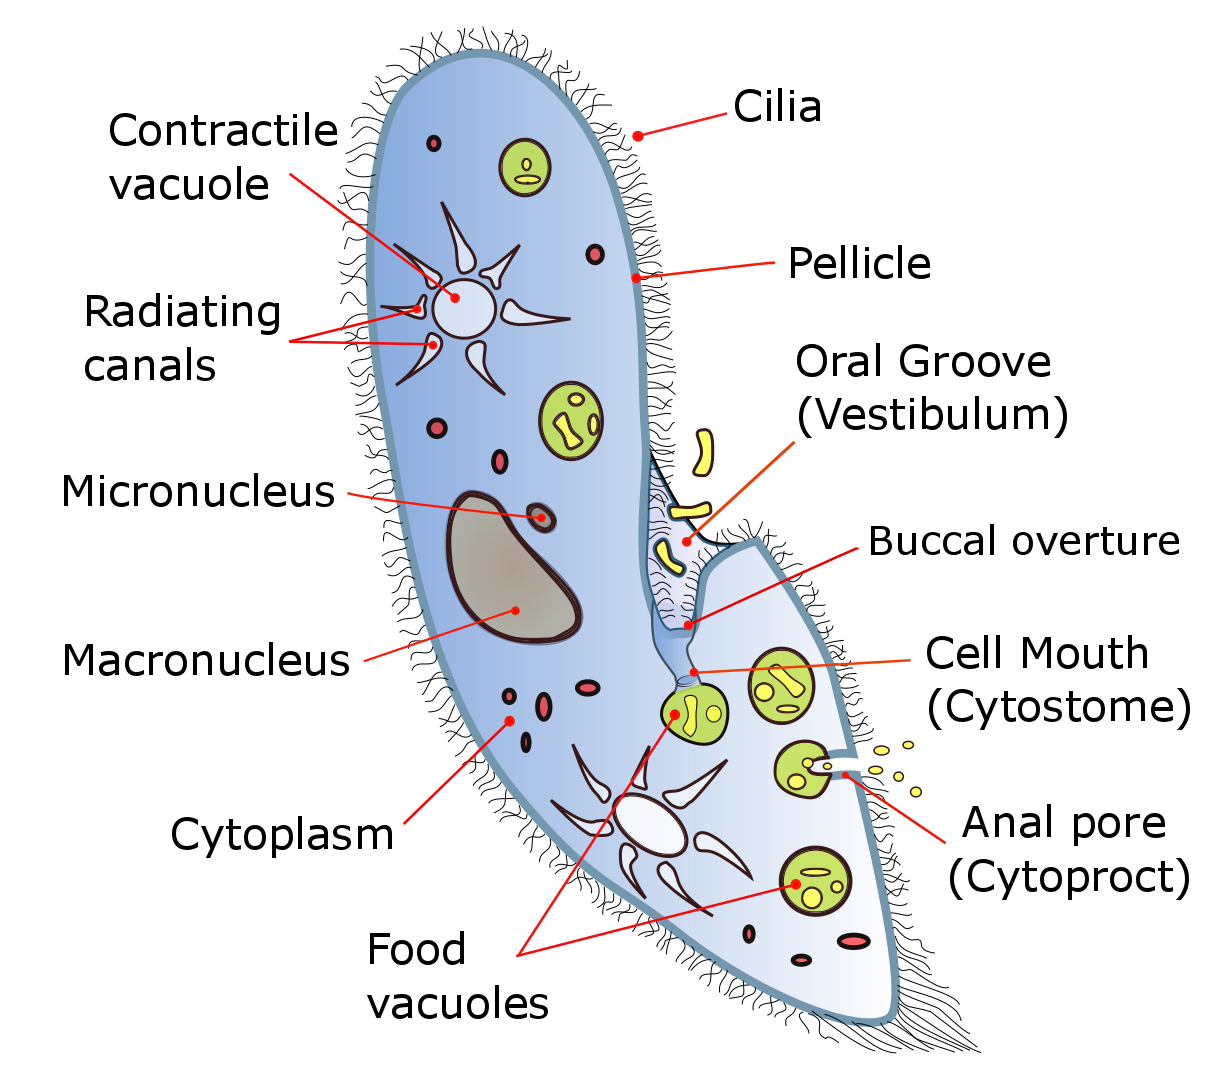
\includegraphics[width=0.7\linewidth]{./figures/protista/Paramecium_diagram} 

}

\caption{\href{https://commons.wikimedia.org/wiki/File:Paramecium_diagram.png}{Diagram of the ciliate Paramecium}}\label{fig:parameciumdiagram}
\end{figure}

Most ciliates are heterotrophs, feeding on smaller organisms, such as bacteria and algae, and detritus swept into the oral groove (mouth) by modified oral cilia. This usually includes a series of membranelles to the left of the mouth and a paroral membrane to its right, both of which arise from polykinetids, groups of many cilia together with associated structures. The food is moved by the cilia through the mouth pore into the gullet, which forms food vacuoles.

Feeding techniques vary considerably, however. Some ciliates are mouthless and feed by absorption (osmotrophy), while others are predatory and feed on other protozoa and in particular on other ciliates. Some ciliates parasitize animals, although only one species, Balantidium coli, is known to cause disease in humans.

Ciliates reproduce asexually, by various kinds of fission. During fission, the micronucleus undergoes mitosis and the macronucleus elongates and undergoes amitosis (except among the Karyorelictean ciliates, whose macronuclei do not divide). The cell then divides in two, and each new cell obtains a copy of the micronucleus and the macronucleus.

Typically, the cell is divided transversally, with the anterior half of the ciliate (the proter) forming one new organism, and the posterior half (the opisthe) forming another. However, other types of fission occur in some ciliate groups. These include budding (the emergence of small ciliated offspring, or ``swarmers'', from the body of a mature parent); strobilation (multiple divisions along the cell body, producing a chain of new organisms); and palintomy (multiple fissions, usually within a cyst).

Fission may occur spontaneously, as part of the vegetative cell cycle. Alternatively, it may proceed as a result of self-fertilization (autogamy), or it may follow conjugation, a sexual phenomenon in which ciliates of compatible mating types exchange genetic material. While conjugation is sometimes described as a form of reproduction, it is not directly connected with reproductive processes, and does not directly result in an increase in the number of individual ciliates or their progeny.

Ciliate conjugation is a sexual phenomenon that results in genetic recombination and nuclear reorganization within the cell. During conjugation, two ciliates of a compatible mating type form a bridge between their cytoplasms. The micronuclei undergo meiosis, the macronuclei disappear, and haploid micronuclei are exchanged over the bridge. In some ciliates (peritrichs, chonotrichs and some suctorians), conjugating cells become permanently fused, and one conjugant is absorbed by the other. In most ciliate groups, however, the cells separate after conjugation, and both form new macronuclei from their micronuclei. Conjugation and autogamy are always followed by fission.



\begin{figure}

{\centering 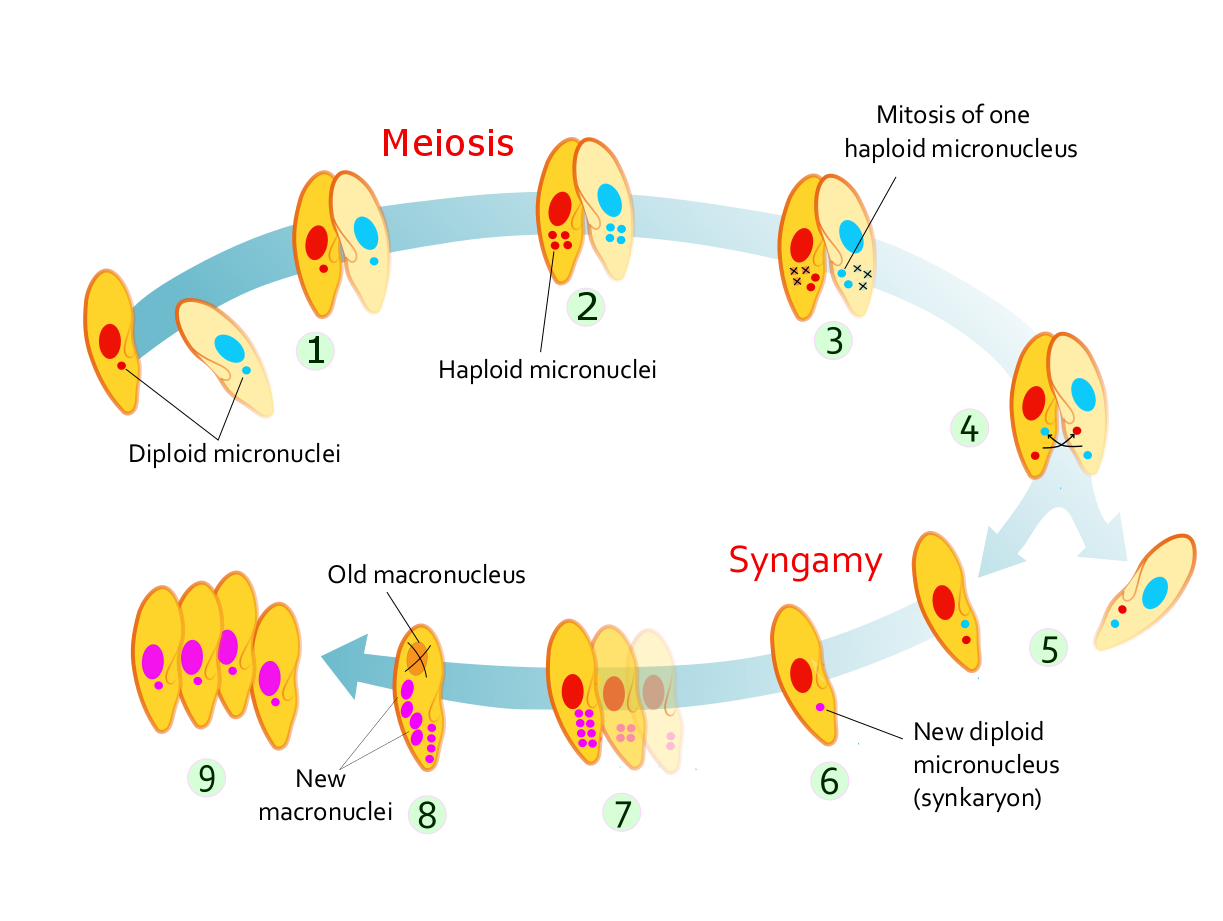
\includegraphics[width=0.7\linewidth]{./figures/protista/Stages_of_ciliate_conjugation} 

}

\caption{\href{https://commons.wikimedia.org/wiki/File:Stages_of_ciliate_conjugation.png}{Stages of conjugation in Paramecium caudatum}}\label{fig:cilconjugation}
\end{figure}

In many ciliates, such as Paramecium, conjugating partners (gamonts) are similar or indistinguishable in size and shape. This is referred to as ``isogamontic'' conjugation. In some groups, partners are different in size and shape. This is referred to as ``anisogamontic'' conjugation. In sessile peritrichs, for instance, one sexual partner (the microconjugant) is small and mobile, while the other (macroconjugant) is large and sessile

In Paramecium caudatum, the stages of conjugation are as follows (see diagram at right):

\begin{enumerate}
\def\labelenumi{\arabic{enumi}.}
\tightlist
\item
  Compatible mating strains meet and partly fuse
\item
  The micronuclei undergo meiosis, producing four haploid micronuclei per cell.
\item
  Three of these micronuclei disintegrate. The fourth undergoes mitosis.
\item
  The two cells exchange a micronucleus.
\item
  The cells then separate.
\item
  The micronuclei in each cell fuse, forming a diploid micronucleus.
\item
  Mitosis occurs three times, giving rise to eight micronuclei.
\item
  Four of the new micronuclei transform into macronuclei, and the old macronucleus disintegrates.
\item
  Binary fission occurs twice, yielding four identical daughter cells.
\end{enumerate}

Ciliates contain two types of nuclei: somatic ``macronucleus'' and the germline ``micronucleus''. Only the DNA in the micronucleus is passed on during sexual reproduction (conjugation). On the other hand, only the DNA in the macronucleus is actively expressed and results in the phenotype of the organism. Macronuclear DNA is derived from micronuclear DNA by amazingly extensive DNA rearrangement and amplification.

The macronucleus begins as a copy of the micronucleus. The micronuclear chromosomes are fragmented into many smaller pieces and amplified to give many copies. The resulting macronuclear chromosomes often contain only a single gene. In Tetrahymena, the micronucleus has 10 chromosomes (five per haploid genome), while the macronucleus has over 20,000 chromosomes.

In addition, the micronuclear genes are interrupted by numerous ``internal eliminated sequences'' (IESs). During development of the macronucleus, IESs are deleted and the remaining gene segments, macronuclear destined sequences (MDSs), are spliced together to give the operational gene. Tetrahymena has about 6,000 IESs and about 15\% of micronuclear DNA is eliminated during this process. The process is guided by small RNAs and epigenetic chromatin marks.

In spirotrich ciliates (such as Oxytricha), the process is even more complex due to ``gene scrambling'': the MDSs in the micronucleus are often in different order and orientation from that in the macronuclear gene, and so in addition to deletion, DNA inversion and translocation are required for ``unscrambling''. This process is guided by long RNAs derived from the parental macronucleus. More than 95\% of micronuclear DNA is eliminated during spirotrich macronuclear development.

\hypertarget{amoebozoa}{%
\section{Amoebozoa}\label{amoebozoa}}

Amoebozoa is a major taxonomic group containing about 2,400 described species of amoeboid protists, often possessing blunt, fingerlike, lobose pseudopods and tubular mitochondrial cristae. In most classification schemes, Amoebozoa is ranked as a phylum within either the kingdom Protista or the kingdom Protozoa. In the classification favored by the International Society of Protistologists, it is retained as an unranked ``supergroup'' within Eukaryota. Molecular genetic analysis supports Amoebozoa as a monophyletic clade. Most phylogenetic trees identify it as the sister group to Opisthokonta, another major clade which contains both fungi and animals as well as some 300 species of unicellular protists. Amoebozoa and Opisthokonta are sometimes grouped together in a high-level taxon, variously named Unikonta, Amorphea or Opimoda.

Amoebozoa includes many of the best-known amoeboid organisms, such as Chaos, Entamoeba, Pelomyxa and the genus Amoeba itself. Species of Amoebozoa may be either shelled (testate), or naked, and cells may possess flagella. Free-living species are common in both salt and freshwater as well as soil, moss and leaf litter. Some live as parasites or symbiotes of other organisms, and some are known to cause disease in humans and other organisms.

While the majority of amoebozoan species are unicellular, the group also includes several varieties of slime molds, which have a macroscopic, multicellular stage of life during which individual amoeboid cells aggregate to produce spores.

Amoebozoa vary greatly in size. Some are only 10--20 μm in diameter, while others are among the largest protozoa. The well-known species Amoeba proteus, which may reach 800 μm in length, is often studied in schools and laboratories as a representative cell or model organism, partly because of its convenient size. Multinucleate amoebae like Chaos and Pelomyxa may be several millimetres in length, and some multicellular amoebozoa, such as the ``dog vomit'' slime mold Fuligo septica, can cover an area of several square meters.

Amoebozoa is a large and diverse group, but certain features are common to many of its members. The amoebozoan cell is typically divided into a granular central mass, called endoplasm, and a clear outer layer, called ectoplasm. During locomotion, the endoplasm flows forwards and the ectoplasm runs backwards along the outside of the cell. In motion, many amoebozoans have a clearly defined anterior and posterior and may assume a ``monopodial'' form, with the entire cell functioning as a single pseudopod. Large pseudopods may produce numerous clear projections called subpseudopodia (or determinate pseudopodia), which are extended to a certain length and then retracted, either for the purpose of locomotion or food intake. A cell may also form multiple indeterminate pseudopodia, through which the entire contents of the cell flow in the direction of locomotion. These are more or less tubular and are mostly filled with granular endoplasm. The cell mass flows into a leading pseudopod, and the others ultimately retract, unless the organism changes direction.

While most amoebozoans are ``naked,'' like the familiar Amoeba and Chaos, or covered with a loose coat of minute scales, like Cochliopodium and Korotnevella, members of the order Arcellinida form rigid shells, or tests, equipped with a single aperture through which the pseudopods emerge. Arcellinid tests may be secreted from organic materials, as in Arcella, or built up from collected particles cemented together, as in Difflugia.

In all amoebozoa, the primary mode of nutrition is phagocytosis, in which the cell surrounds potential food particles with its pseudopods, sealing them into vacuoles within which they may be digested and absorbed. Some amoebozoans have a posterior bulb called a uroid, which may serve to accumulate waste, periodically detaching from the rest of the cell.{[}citation needed{]} When food is scarce, most species can form cysts, which may be carried aerially and introduce them to new environments.{[}citation needed{]} In slime moulds, these structures are called spores, and form on stalked structures called fruiting bodies or sporangia.

The majority of Amoebozoa lack flagella and more generally do not form microtubule-supported structures except during mitosis. However, flagella do occur among the Archamoebae, and many slime moulds produce biflagellate gametes{[}citation needed{]}. The flagellum is generally anchored by a cone of microtubules, suggesting a close relationship to the opisthokonts.{[}citation needed{]} The mitochondria in amoebozoan cells characteristically have branching tubular cristae. However, among the Archamoebae, which are adapted to anoxic or microaerophilic habitats, mitochondria have been lost.

Amoebiasis, also known as amebiasis or entamoebiasis, is an infection caused by any of the amoebozoans of the Entamoeba group. Symptoms are most common upon infection by Entamoeba histolytica. Amoebiasis can present with no, mild, or severe symptoms. Symptoms may include abdominal pain, mild diarrhoea, bloody diarrhea or severe colitis with tissue death and perforation. This last complication may cause peritonitis. People affected may develop anemia due to loss of blood.

Invasion of the intestinal lining causes amoebic bloody diarrhea or amoebic colitis. If the parasite reaches the bloodstream it can spread through the body, most frequently ending up in the liver where it causes amoebic liver abscesses. Liver abscesses can occur without previous diarrhea. Cysts of Entamoeba can survive for up to a month in soil or for up to 45 minutes under fingernails. It is important to differentiate between amoebiasis and bacterial colitis. The preferred diagnostic method is through faecal examination under microscope, but requires a skilled microscopist and may not be reliable when excluding infection. This method however may not be able to separate between specific types. Increased white blood cell count is present in severe cases, but not in mild ones. The most accurate test is for antibodies in the blood, but it may remain positive following treatment.

Prevention of amoebiasis is by separating food and water from faeces and by proper sanitation measures. There is no vaccine. There are two treatment options depending on the location of the infection. Amoebiasis in tissues is treated with either metronidazole, tinidazole, nitazoxanide, dehydroemetine or chloroquine, while luminal infection is treated with diloxanide furoate or iodoquinoline. For treatment to be effective against all stages of the amoeba may require a combination of medications. Infections without symptoms do not require treatment but infected individuals can spread the parasite to others and treatment can be considered. Treatment of other Entamoeba infections apart from E. histolytica is not needed.

Amoebiasis is present all over the world. About 480 million people are infected with what appears to be E. histolytica and these result in the death of between 40,000--110,000 people every year. Most infections are now ascribed to E. dispar. E. dispar is more common in certain areas and symptomatic cases may be fewer than previously reported. The first case of amoebiasis was documented in 1875 and in 1891 the disease was described in detail, resulting in the terms amoebic dysentery and amoebic liver abscess. Further evidence from the Philippines in 1913 found that upon ingesting cysts of E. histolytica volunteers developed the disease. It has been known since 1897 that at least one non-disease-causing species of Entamoeba existed (Entamoeba coli), but it was first formally recognized by the WHO in 1997 that E. histolytica was two species, despite this having first been proposed in 1925. In addition to the now-recognized E. dispar evidence shows there are at least two other species of Entamoeba that look the same in humans - E. moshkovskii and Entamoeba bangladeshi. The reason these species haven't been differentiated until recently is because of the reliance on appearance.

\hypertarget{algae}{%
\section{Algae}\label{algae}}

The Archaeplastida (or kingdom Plantae sensu lato) are a major group of autotrophic eukaryotes, comprising the red algae (Rhodophyta), the green algae, and the land plants, together with a small group of freshwater unicellular algae called glaucophytes. The Archaeplastida have chloroplasts that are surrounded by two membranes, suggesting that they were acquired directly from endosymbiotic cyanobacteria. All other groups besides the amoeboid Paulinella chromatophora, have chloroplasts surrounded by three or four membranes, suggesting they were acquired secondarily from red or green algae. Unlike red and green algae, glaucophytes have never been involved in secondary endosymbiosis events.

The cells of the Archaeplastida typically lack centrioles and have mitochondria with flat cristae. They usually have a cell wall that contain cellulose, and food is stored in the form of starch. However, these characteristics are also shared with other eukaryotes. The main evidence that the Archaeplastida form a monophyletic group comes from genetic studies, which indicate their plastids probably had a single origin. This evidence is disputed. Based on the evidence to date, it is not possible to confirm or refute alternative evolutionary scenarios to a single primary endosymbiosis. Photosynthetic organisms with plastids of different origin (such as brown algae) do not belong to the Archaeplastida.

The archaeplastidans fall into two main evolutionary lines. The red algae are pigmented with chlorophyll a and phycobiliproteins, like most cyanobacteria, and accumulate starch outside the chloroplasts. The green algae and land plants -- together known as Viridiplantae (Latin for ``green plants'') or Chloroplastida -- are pigmented with chlorophylls a and b, but lack phycobiliproteins, and starch is accumulated inside the chloroplasts. The glaucophytes have typical cyanobacterial pigments, and are unusual in retaining a cell wall within their plastids (called cyanelles).

\href{https://en.wikipedia.org/wiki/Algae}{Algae} is an informal term for a large and diverse group of photosynthetic eukaryotic organisms. It is a polyphyletic grouping, including species from multiple distinct clades. Included organisms range from unicellular microalgae, such as Chlorella and the diatoms, to multicellular forms, such as the giant kelp, a large brown alga which may grow up to 50 m in length. Most are aquatic and autotrophic and lack many of the distinct cell and tissue types, such as stomata, xylem and phloem, which are found in land plants. The largest and most complex marine algae are called seaweeds, while the most complex freshwater forms are the Charophyta, a division of green algae which includes, for example, Spirogyra and stoneworts.



\begin{figure}

{\centering 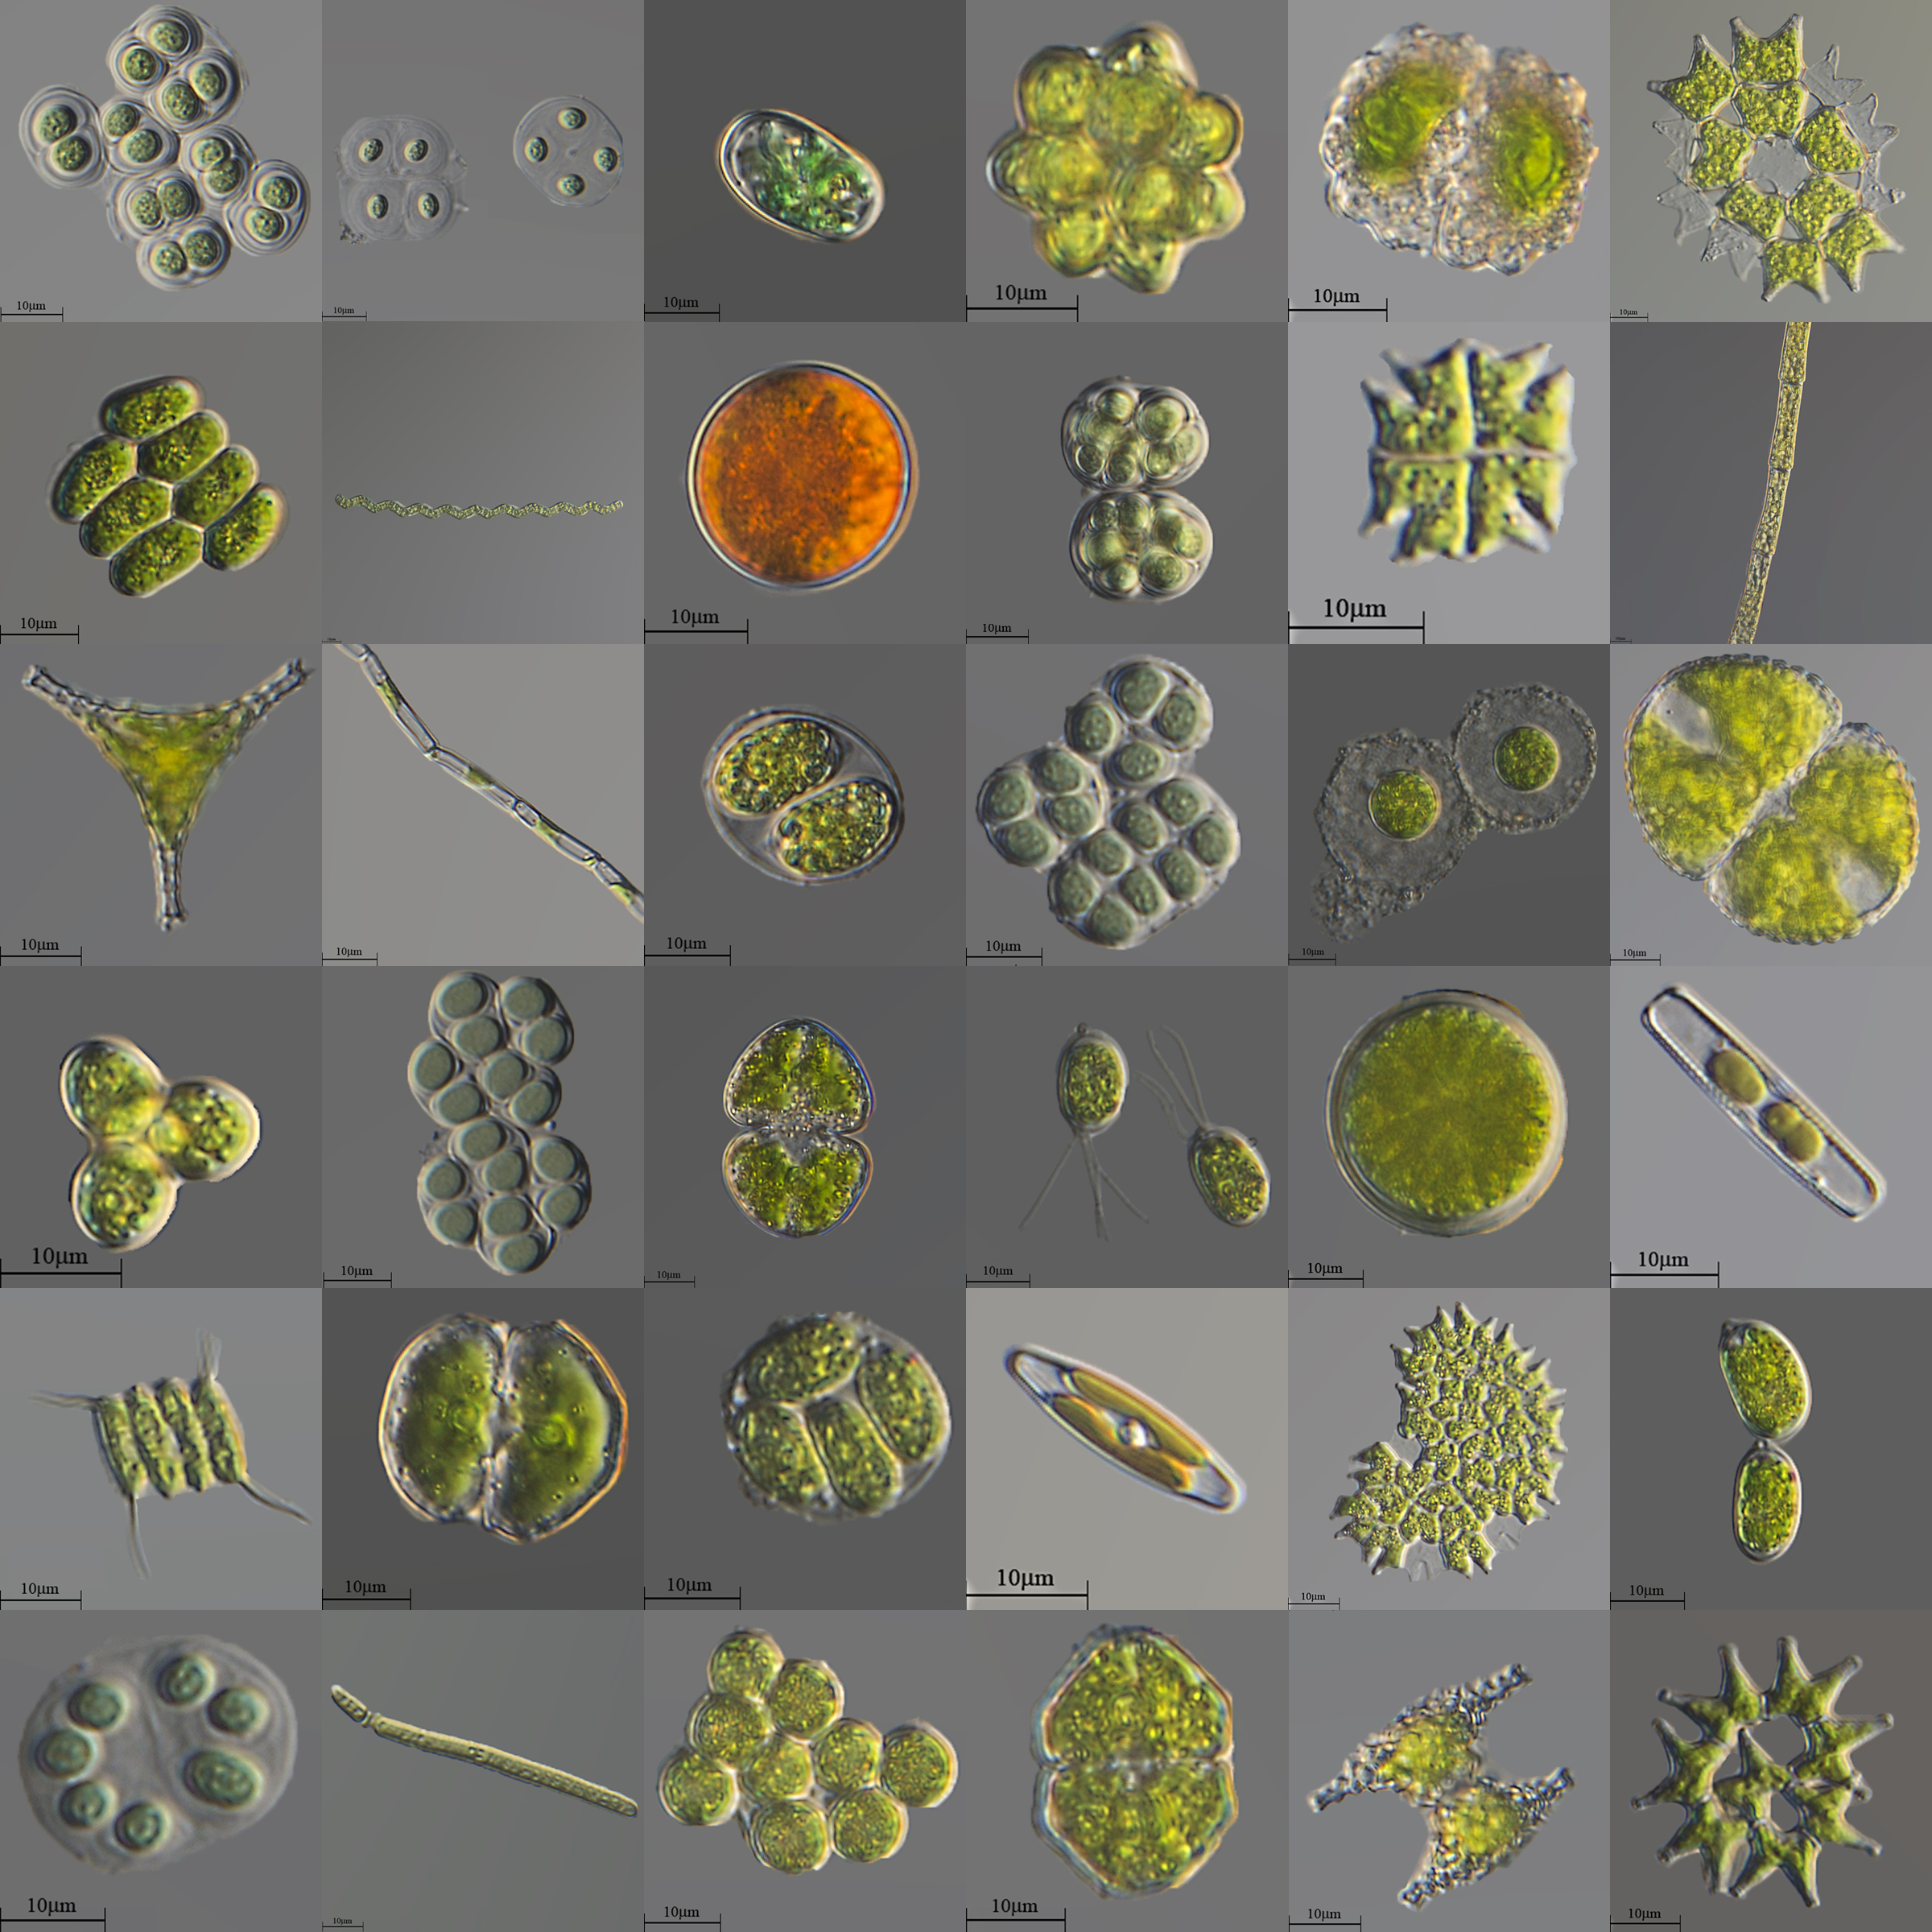
\includegraphics[width=0.7\linewidth]{./figures/protista/algae_collection} 

}

\caption{\href{https://commons.wikimedia.org/wiki/File:Водоросли_пресноводного_водоема.jpg}{A variety of microscopic unicellular and colonial freshwater algae}}\label{fig:algaecollection}
\end{figure}

No definition of algae is generally accepted. One definition is that algae ``have chlorophyll as their primary photosynthetic pigment and lack a sterile covering of cells around their reproductive cells''. Although cyanobacteria are often referred to as ``blue-green algae'', most authorities exclude all prokaryotes from the definition of algae.

Algae constitute a polyphyletic group since they do not include a common ancestor, and although their plastids seem to have a single origin, from cyanobacteria, they were acquired in different ways. Green algae are examples of algae that have primary chloroplasts derived from endosymbiotic cyanobacteria. Diatoms and brown algae are examples of algae with secondary chloroplasts derived from an endosymbiotic red alga.

Algae exhibit a wide range of reproductive strategies, from simple asexual cell division to complex forms of sexual reproduction.



\begin{figure}

{\centering 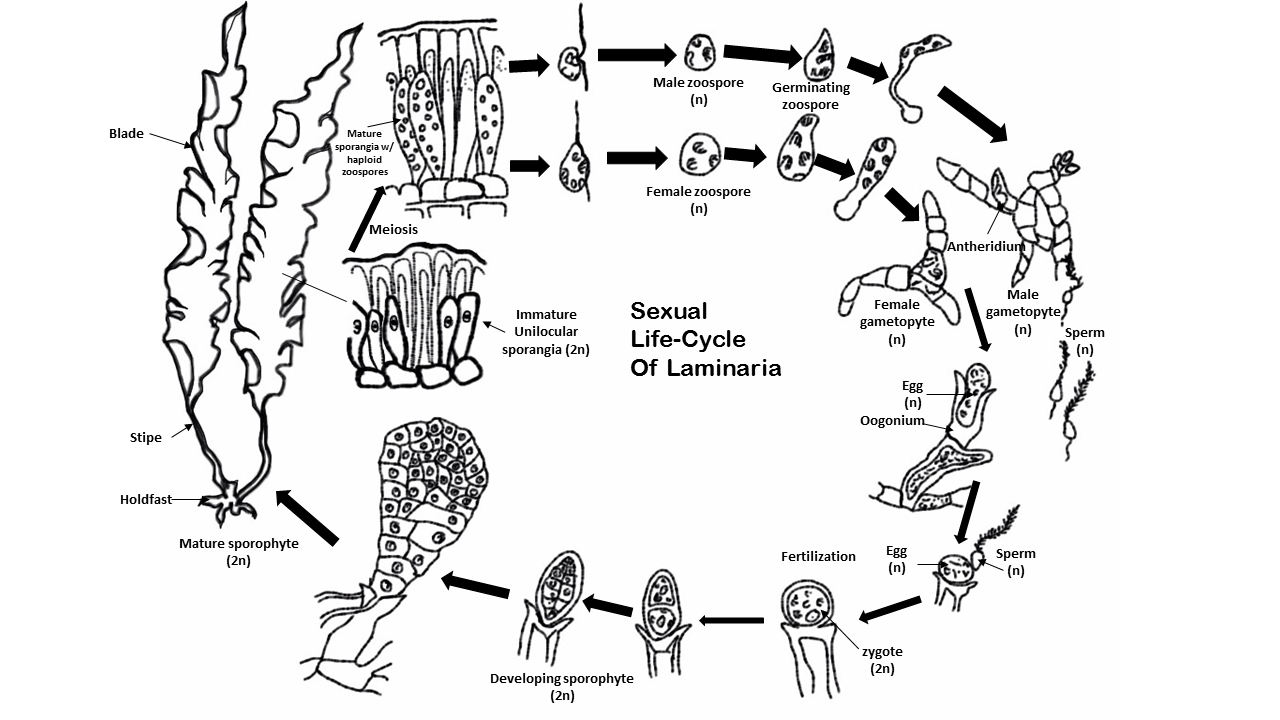
\includegraphics[width=0.7\linewidth]{./figures/protista/Laminaria_Life_Cycle} 

}

\caption{\href{https://commons.wikimedia.org/wiki/File:Laminaria_Life_Cycle.png}{The sexual life cycle of Laminaria, a representative of some 30 different species of brown algae that are commonly called ``kelp''.}}\label{fig:laminarialifecycle}
\end{figure}

Algae lack the various structures that characterize land plants, such as the phyllids (leaf-like structures) of bryophytes, rhizoids in nonvascular plants, and the roots, leaves, and other organs found in tracheophytes (vascular plants). Most are phototrophic, although some are mixotrophic, deriving energy both from photosynthesis and uptake of organic carbon either by osmotrophy, myzotrophy, or phagotrophy. Some unicellular species of green algae, many golden algae, euglenids, dinoflagellates, and other algae have become heterotrophs (also called colorless or apochlorotic algae), sometimes parasitic, relying entirely on external energy sources and have limited or no photosynthetic apparatus. Some other heterotrophic organisms, such as the apicomplexans, are also derived from cells whose ancestors possessed plastids, but are not traditionally considered as algae. Algae have photosynthetic machinery ultimately derived from cyanobacteria that produce oxygen as a by-product of photosynthesis, unlike other photosynthetic bacteria such as purple and green sulfur bacteria. Fossilized filamentous algae from the Vindhya basin have been dated back to 1.6 to 1.7 billion years ago.

The first land plants probably evolved from shallow freshwater charophyte algae much like Chara almost 500 million years ago. These probably had an isomorphic alternation of generations and were probably filamentous. Fossils of isolated land plant spores suggest land plants may have been around as long as 475 million years ago.

Most of the simpler algae are unicellular flagellates or amoeboids, but colonial and nonmotile forms have developed independently among several of the groups.

In three lines of algae, even higher levels of organization have been reached, with full tissue differentiation. These are the brown algae,---some of which may reach 50 m in length (kelps)---the red algae, and the green algae. The most complex forms are found among the charophyte algae (see Charales and Charophyta), in a lineage that eventually led to the higher land plants. The innovation that defines these nonalgal plants is the presence of female reproductive organs with protective cell layers that protect the zygote and developing embryo. Hence, the land plants are referred to as the Embryophytes.

Rhodophyta, Chlorophyta, and Heterokontophyta, the three main algal divisions, have lifecycles which show considerable variation and complexity. In general, an asexual phase exists where the seaweed's cells are diploid, a sexual phase where the cells are haploid, followed by fusion of the male and female gametes. Asexual reproduction permits efficient population increases, but less variation is possible. Commonly, in sexual reproduction of unicellular and colonial algae, two specialized, sexually compatible, haploid gametes make physical contact and fuse to form a zygote. To ensure a successful mating, the development and release of gametes is highly synchronized and regulated; pheromones may play a key role in these processes. Meiosis has been shown to occur in many different species of algae.

For example, Fucus is a genus of brown algae found in the intertidal zones of rocky seashores almost throughout the world. Species of Fucus are recorded almost worldwide. They are dominant on the shores of the British Isles, the northeastern coast of North America and California. These algae have a relatively simple life cycle and produce only one type of thallus which grows to a maximum size of 2 m. Fertile cavities, the conceptacles, containing the reproductive cells are immersed in the receptacles near the ends of the branches. After meiosis oogonia and antheridia, the female and male reproductive organs, produce egg cells and sperm respectively that are released into the sea where fertilisation takes place. The resulting zygote develops directly into the diploid plant. This contrasts with the life cycle of the flowering plant, where the egg cells and sperm are produced by a haploid multicellular generation, albeit very strongly reduced, and the egg cells are fertilised within the ovules of the parent plant and then released as seeds.

Algae are prominent in bodies of water, common in terrestrial environments, and are found in unusual environments, such as on snow and ice. Seaweeds grow mostly in shallow marine waters, under 100 m (330 ft) deep; however, some such as Navicula pennata have been recorded to a depth of 360 m (1,180 ft). A type of algae, Ancylonema nordenskioeldii, was found in Greenland in areas known as the `Dark Zone', which caused an increase in the rate of melting ice sheet. Same algae was found in the Italian Alps, after pink ice appeared on parts of the Presena glacier.

The various sorts of algae play significant roles in aquatic ecology. Microscopic forms that live suspended in the water column (phytoplankton) provide the food base for most marine food chains. In very high densities (algal blooms), these algae may discolor the water and outcompete, poison, or asphyxiate other life forms.

\hypertarget{slime-molds}{%
\section{Slime Molds}\label{slime-molds}}

Slime mold or slime mould is an informal name given to several kinds of unrelated eukaryotic organisms that can live freely as single cells, but can aggregate together to form multicellular reproductive structures. Slime molds were formerly classified as fungi but are no longer considered part of that kingdom. Although not forming a single monophyletic clade, they are grouped within the paraphyletic group referred to as kingdom Protista.

More than 900 species of slime mold occur globally. Their common name refers to part of some of these organisms' life cycles where they can appear as gelatinous ``slime''. This is mostly seen with the Myxogastria, which are the only macroscopic slime molds. Most slime molds are smaller than a few centimeters, but some species may reach sizes up to several square meters and masses up to 20 kilograms.

Many slime molds, mainly the ``cellular'' slime molds, do not spend most of their time in this state. When food is abundant, these slime molds exist as single-celled organisms. When food is in short supply, many of these single-celled organisms will congregate and start moving as a single body. In this state they are sensitive to airborne chemicals and can detect food sources. They can readily change the shape and function of parts, and may form stalks that produce fruiting bodies, releasing countless spores, light enough to be carried on the wind or hitch a ride on passing animals.

They feed on microorganisms that live in any type of dead plant material. They contribute to the decomposition of dead vegetation, and feed on bacteria, yeasts, and fungi. For this reason, slime molds are usually found in soil, lawns, and on the forest floor, commonly on deciduous logs. In tropical areas they are also common on inflorescences and fruits, and in aerial situations (e.g., in the canopy of trees). In urban areas, they are found on mulch or in the leaf mold in rain gutters, and also grow in air conditioners, especially when the drain is blocked.

Slime molds begin life as amoeba-like cells. These unicellular amoebae are commonly haploid and feed on bacteria. These amoebae can mate if they encounter the correct mating type and form zygotes that then grow into plasmodia. These contain many nuclei without cell membranes between them, and can grow to meters in size. The species Fuligo septica is often seen as a slimy yellow network in and on rotting logs. The amoebae and the plasmodia engulf microorganisms. The plasmodium grows into an interconnected network of protoplasmic strands.



\begin{figure}

{\centering 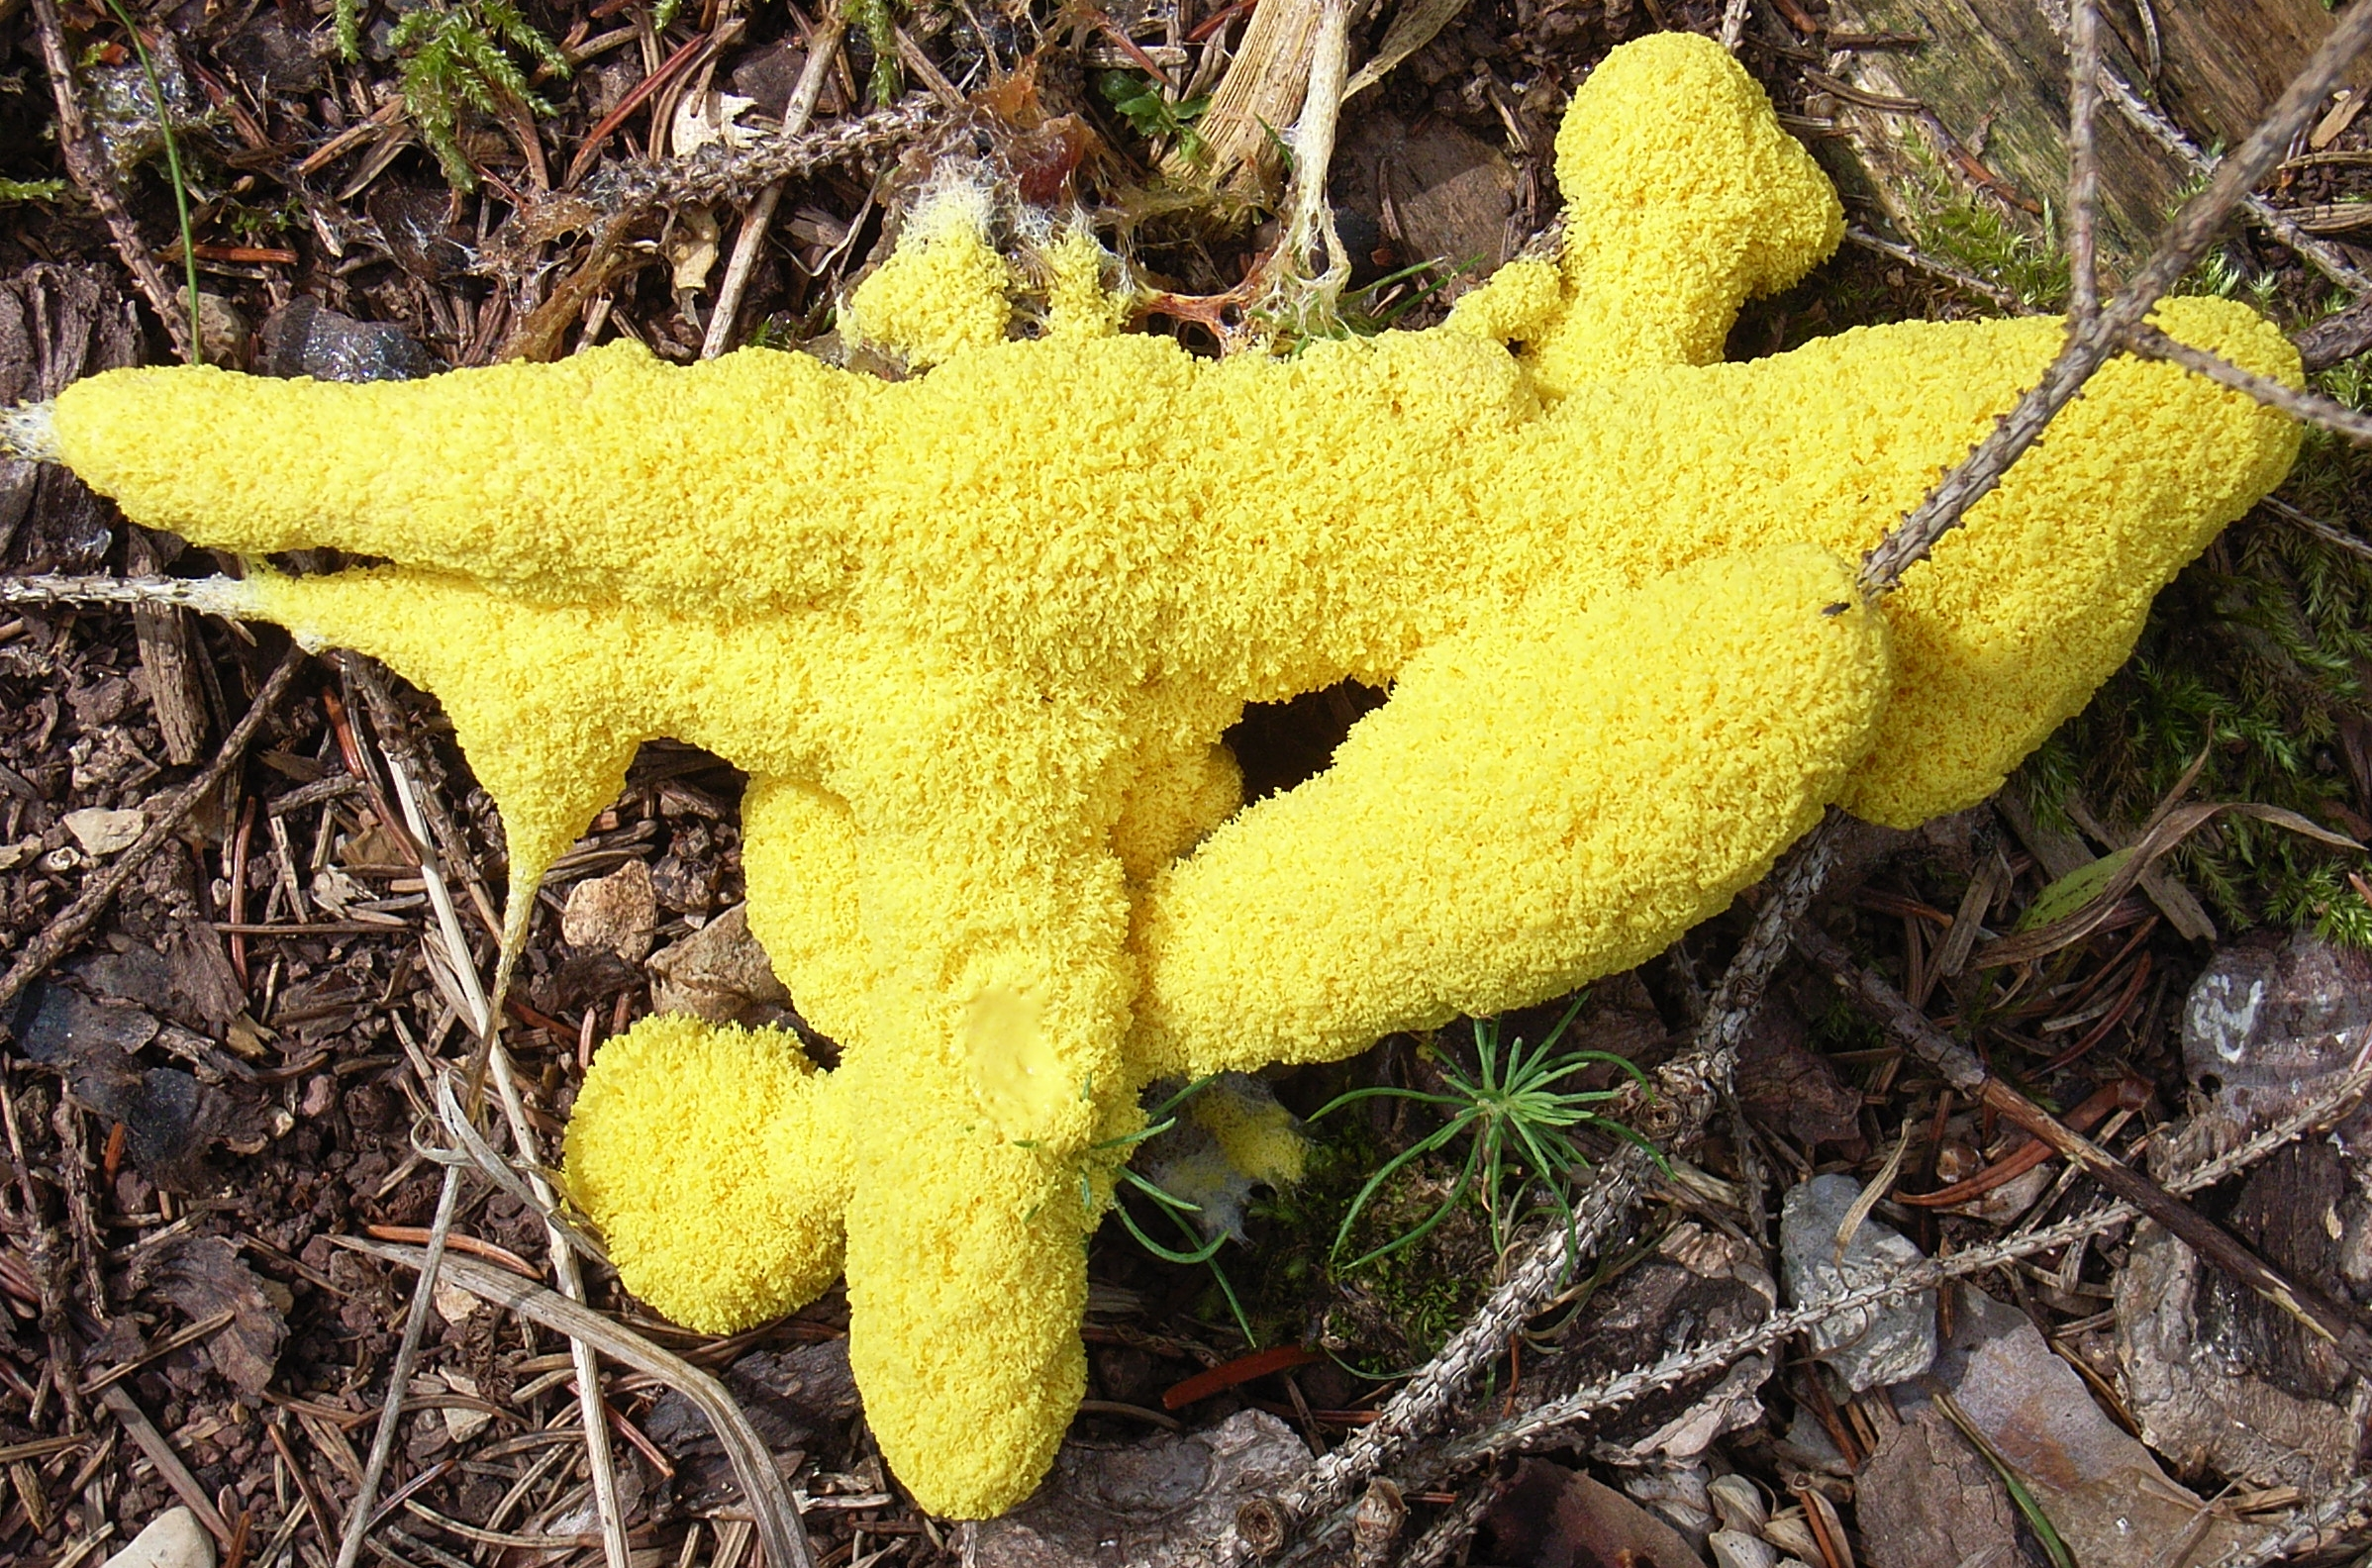
\includegraphics[width=0.7\linewidth]{./figures/protista/Fuligo_septica_bl1} 

}

\caption{\href{https://commons.wikimedia.org/wiki/File:Fuligo_septica_bl1.JPG}{Fuligo septica, a slime mold} Fuligo septica is a species of plasmodial slime mold, and a member of the Myxomycetes class. It is commonly known as the scrambled egg slime, or flowers of tan because of its peculiar yellowish, bile-colored appearance. Also known as the dog vomit slime mold, it is common with a worldwide distribution, and it is often found on bark mulch in urban areas after heavy rain or excessive watering. Their spores are produced on or in aerial sporangia and are spread by wind.}\label{fig:fuligo}
\end{figure}

Within each protoplasmic strand, the cytoplasmic contents rapidly stream. If one strand is carefully watched for about 50 seconds, the cytoplasm can be seen to slow, stop, and then reverse direction. The streaming protoplasm within a plasmodial strand can reach speeds of up to 1.35 mm per second, which is the fastest rate recorded for any microorganism. Migration of the plasmodium is accomplished when more protoplasm streams to advancing areas and protoplasm is withdrawn from rear areas. When the food supply wanes, the plasmodium will migrate to the surface of its substrate and transform into rigid fruiting bodies. The fruiting bodies or sporangia are what are commonly seen. They superficially look like fungi or molds but are not related to the true fungi. These sporangia will then release spores which hatch into amoebae to begin the life cycle again.



\begin{figure}

{\centering 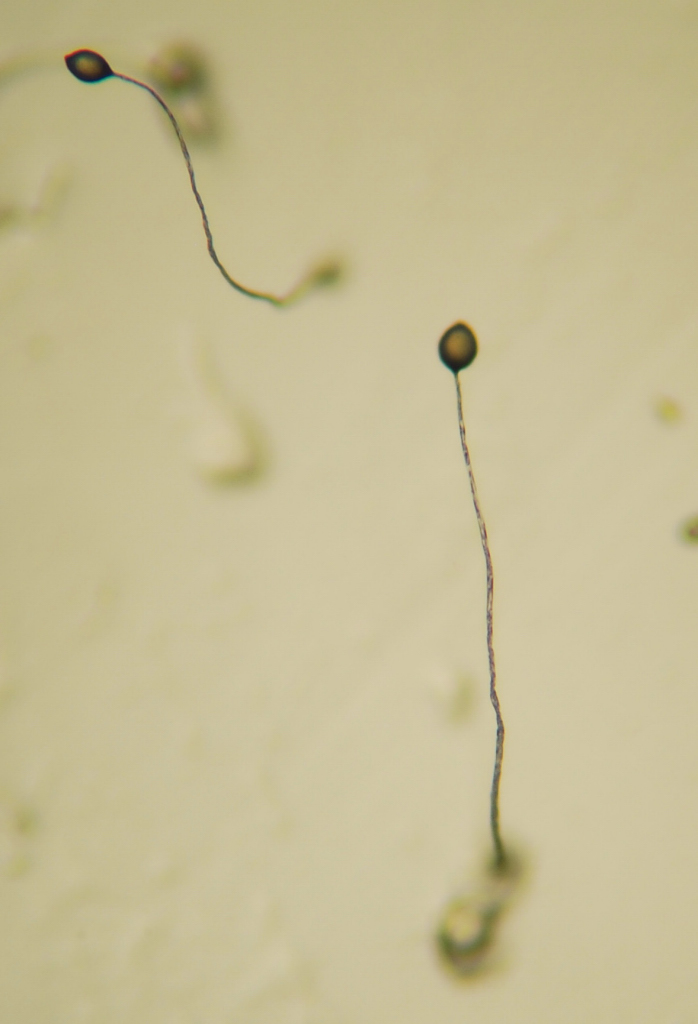
\includegraphics[width=0.7\linewidth]{./figures/protista/Dictyostelium_Fruiting_Bodies} 

}

\caption{\href{https://commons.wikimedia.org/wiki/File:Dictyostelium_Fruiting_Bodies.JPG}{Dictyostelium Fruiting Body} Dictyostelium is a genus of single- and multi-celled eukaryotic, phagotrophic bacterivores. Though they are Protista and in no way fungal, they traditionally are known as ``slime molds''. They are present in most terrestrial ecosystems as a normal and often abundant component of the soil microflora, and play an important role in the maintenance of balanced bacterial populations in soils.}\label{fig:dictfruiting}
\end{figure}



\begin{figure}

{\centering 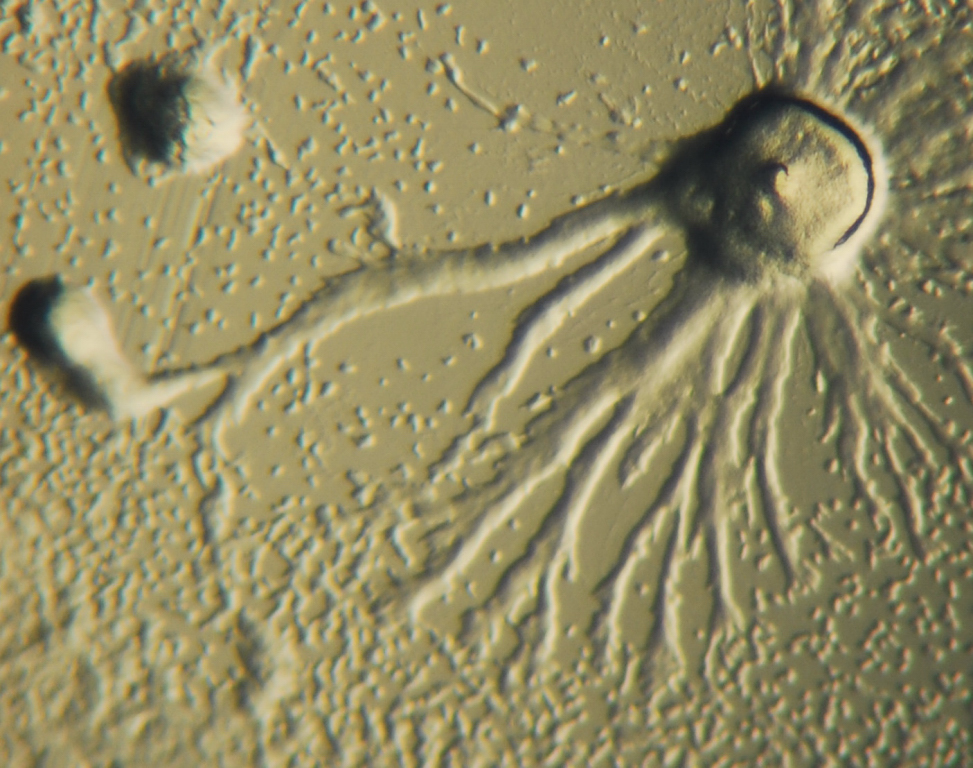
\includegraphics[width=0.7\linewidth]{./figures/protista/Dictyostelium_Aggregation} 

}

\caption{\href{https://commons.wikimedia.org/wiki/File:Dictyostelium_Aggregation.JPG}{Dictyostelium colony in process of aggregation}}\label{fig:dictformcol}
\end{figure}



\begin{figure}

{\centering 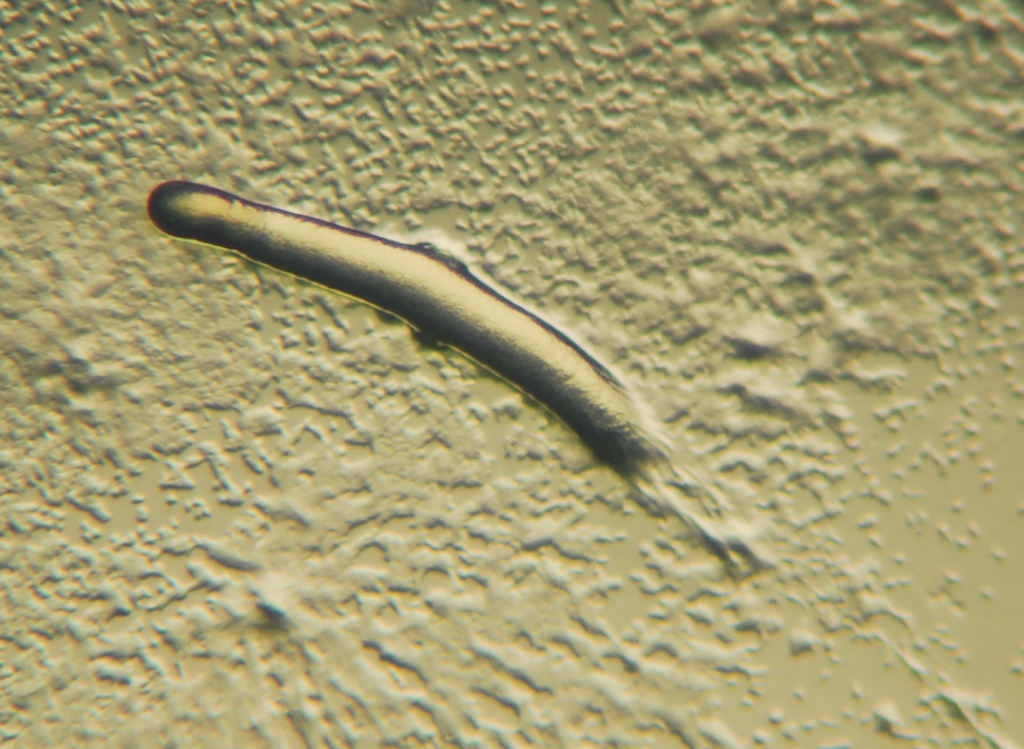
\includegraphics[width=0.7\linewidth]{./figures/protista/Dictyostelium_Pseudoplasmodium} 

}

\caption{\href{https://commons.wikimedia.org/wiki/File:Dictyostelium_Pseudoplasmodium.JPG}{Pseudoplasmodium or ``slug'' of a Dictyostelium}}\label{fig:dictslug}
\end{figure}

\hypertarget{reproduction-of-protists}{%
\subsection{Reproduction of Protists}\label{reproduction-of-protists}}

Some protists reproduce sexually using gametes, while others reproduce asexually.

Some species, for example \emph{Plasmodium falciparum,} have extremely complex life cycles that involve multiple forms of the organism, some of which reproduce sexually and others asexually. However, it is unclear how frequently sexual reproduction causes genetic exchange between different strains of Plasmodium in nature and most populations of parasitic protists may be clonal lines that rarely exchange genes with other members of their species.

Eukaryotes emerged in evolution more than 1.5 billion years ago. The earliest eukaryotes were likely protists. Although sexual reproduction is widespread among extant eukaryotes, it seemed unlikely until recently, that sex could be a primordial and fundamental characteristic of eukaryotes. A principal reason for this view was that sex appeared to be lacking in certain pathogenic protists whose ancestors branched off early from the eukaryotic family tree. However, several of these protists are now known to be capable of, or to recently have had the capability for, meiosis and hence sexual reproduction. For example, the common intestinal parasite Giardia lamblia was once considered to be a descendant of a protist lineage that predated the emergence of meiosis and sex. However, G. lamblia was recently found to have a core set of genes that function in meiosis and that are widely present among sexual eukaryotes. These results suggested that G. lamblia is capable of meiosis and thus sexual reproduction. Furthermore, direct evidence for meiotic recombination, indicative of sex, was also found in G. lamblia.

The pathogenic parasitic protists of the genus Leishmania have been shown to be capable of a sexual cycle in the invertebrate vector, likened to the meiosis undertaken in the trypanosomes.

Protists generally reproduce asexually under favorable environmental conditions, but tend to reproduce sexually under stressful conditions, such as starvation or heat shock. Oxidative stress, which is associated with the production of reactive oxygen species leading to DNA damage, also appears to be an important factor in the induction of sex in protists.

Some commonly found Protist pathogens such as \emph{Toxoplasma gondii} are capable of infecting and undergoing asexual reproduction in a wide variety of animals -- which act as secondary or intermediate host -- but can undergo sexual reproduction only in the primary or definitive host (for example: felids such as domestic cats in this case).

Free-living Protists occupy almost any environment that contains liquid water. Many protists, such as algae, are photosynthetic and are vital primary producers in ecosystems, particularly in the ocean as part of the plankton. Protists make up a large portion of the biomass in both marine and terrestrial environments.

Other protists include pathogenic species, such as the kinetoplastid Trypanosoma brucei, which causes sleeping sickness, and species of the apicomplexan Plasmodium, which cause malaria.

Some protists are significant parasites of animals (e.g.; five species of the parasitic genus Plasmodium cause malaria in humans and many others cause similar diseases in other vertebrates), plants (the oomycete Phytophthora infestans causes late blight in potatoes) or even of other protists. Protist pathogens share many metabolic pathways with their eukaryotic hosts. This makes therapeutic target development extremely difficult -- a drug that harms a protist parasite is also likely to harm its animal/plant host. A more thorough understanding of protist biology may allow these diseases to be treated more efficiently. For example, the apicoplast (a nonphotosynthetic chloroplast but essential to carry out important functions other than photosynthesis) present in apicomplexans provides an attractive target for treating diseases caused by dangerous pathogens such as plasmodium.


